\documentclass[11pt]{amsart}
\usepackage{geometry}                % See geometry.pdf to learn the layout options. There are lots.
\geometry{letterpaper}                   % ... or a4paper or a5paper or ... 
%\geometry{landscape}                % Activate for for rotated page geometry
%\usepackage[parfill]{parskip}    % Activate to begin paragraphs with an empty line rather than an indent
\usepackage{graphicx}
\usepackage{amssymb}
\usepackage{epstopdf}
\DeclareGraphicsRule{.tif}{png}{.png}{`convert #1 `dirname #1`/`basename #1 .tif`.png}

\title{Simulation of elastic media with cell contraction in Netgen}
\author{}
%\date{}                                           % Activate to display a given date or no date

\begin{document}
\maketitle



\section{Theory: variational formulation of linear isotropic elasticity with a cellular contraction component}

\subsection{Basic linear elasticity}

Basic linear elasticity is very well-known\cite{bower_applied_2010,slaughter_linearized_2002}, we repeat here merely the main equations for the readers convenience and further developments. In linear small deformation elasticity, the symmetric deformation tensor is:

\begin{equation}
\epsilon_{ij}=\frac{1}{2}\left(\frac{\partial u_i}{\partial x_j}+\frac{\partial u_j}{\partial x_i}\right) \label{eq_deformation_tensor}
\end{equation}

where $x$ designates the spatial coordinates, and $u$ the local deformation field. $i$ and $j$ are indices over the 3 spatial directions (i.e. $u_1=u_x$, $u_2=u_y$ and $u_3=u_z$; $x_1=x$, $x_2=y$ and $x_3=z$ when using conventional notation ).

Solid-body rotations would lead to antisymmetric components in $\epsilon_{ij}$, however, since static solid-body rotations do not lead development of stress in classical continuum mechanics, one considers only the symmetric formulation given by eq. \ref{eq_deformation_tensor}.  

Regarding signs, eq. \ref{eq_deformation_tensor} follows the solid-mechanics convention: if a material is stretched along a given direction $x_i$, the corresponding derivative $\left(\frac{\partial u_i}{\partial x_i} \right)$ and therefore the corresponding entry $\left(\epsilon_{ii}\right)$ is positive. 

In basic linear elasticity\cite{slaughter_linearized_2002}, the deformation field is accompanied by a corresponding stress tensor field $\sigma_{ij}$:

\begin{equation}
\sigma_{ij}=C_{ijkl}\epsilon_{kl} \label{C_stress_tensor}
\end{equation}

where $C_{ijkl}$ denotes the set of proportionality constants. Here, the Einstein summation convention is used, which states that one sums over recurring indexes, which are here $k$ and $l$. In the absence of internal degrees of rotational freedom, $\sigma_{ij}$ is symmetric as well\cite{mclennan_symmetry_1966} and

\begin{equation}
\sigma_{ij}=\sigma_{ji}
\end{equation}

holds.

We consider first the basic case of quasistatic linear elasticity, before explicitly adding the cell contraction forces. In the quasistatic case, acceleration terms are negligeable and the stress tensor field is in equilibrium with external forces:

\begin{equation}
\frac{\partial \sigma_{ij}}{\partial x_j}+s_i = 0 \label{eq_force_balance}
\end{equation}

where the $s_i$ are the spatial components indexed by $i$ of externally applied local force densities.

\subsection{Variational formulation}

Although concise, the mathematical difficulty with eq. \ref{eq_force_balance} is that is is a second order partial differential equation. The gradient of the stress tensor indeed introduces a first step of derivation, but the $\sigma_{ij}$ depend already on the gradients of the deformation field (through eq. \ref{eq_deformation_tensor}). For finite element simulation, it is difficult to find a unique solution to such a second order partial, while better algorithms are known for optimization problems. For this reason, the "weak" or variational formulations have been introduced\cite{bower_applied_2010}. The idea is to use a combination of trial function approach and partial integration\cite{bower_applied_2010}.  

To do so, one forms the scalar product of the zero-valued right-hand side vector given by eq. \ref{eq_force_balance} with an arbitrary trial vector function $v_i$: 

\begin{equation}
\left(\frac{\partial \sigma_{ij}}{\partial x_j}+s_i \right) v_i = 0 \label{eq_trial_function}
\end{equation}

Eq. \ref{eq_force_balance} obviously implies eq. \ref{eq_trial_function} since multiplication of a zero with any finite value yields zero. But due to the arbitraryness of $v_i$, the converse is true too by the Lax-Milgrem theorem\cite{lax_ix_2016}. This realization with trial functions is the basis of the so-called weak formulations\cite{bower_applied_2010}.

In order to reduce the order of the derivatives, one then uses partial integration over a domain $\Omega$, in conjunction with the divergence theorem allowing to interconvert between surface and volume integrals:

\begin{equation}
\int_\Omega \frac{\partial \sigma_{ij}}{\partial x_j}v_i\text{d}V+\int_\Omega s_i v_i \text{d}V=0 \label{eq_int_0}
\end{equation}

with again the Lax-Milgrem theorem\cite{lax_ix_2016} ensuring that under reasonable conditions, eq. \ref{eq_int_0} implies eq. \ref{eq_force_balance}.

Applying the divergence theorem between surface and volume integrals, and using partial integration, one obtains:
\begin{equation}
\int_\Omega \sigma_{ij} \frac{\partial v_i}{\partial x_j} \text{d}V=\int_\Omega s_i v_i \text{d}V+\int_{\delta\Omega} \sigma_{ij}v_i\text{d}S_j 
\end{equation}

One then notes that the surface forces $f_{\text{S}}$ must match the strain tensor at the boundary of the domain under consideration $\delta\Omega$. Further, given the symmetric nature of the stress tensor in standard linear elastics, only the symmetric part of the gradient tensor of the trial function $v$ is relevant. Therefore, this becomes the classical weak formulation\cite{bower_applied_2010}:

\begin{equation}
\int_\Omega \sigma_{ij}\cdot \left(\epsilon_v\right)_{ij}  \text{d}V=\int_\Omega s_i v_i \text{d}V+\int_{\delta\Omega} v_i\text{d}f_{\text{S,}i} \label{eq_variational}
\end{equation}

where

\begin{equation}
\left(\epsilon_v\right)_{ij}=\frac{1}{2}\left(\frac{\partial v_i}{\partial x_j} +\frac{\partial v_j}{\partial x_i}\right) \label{eq_v_deformation_tensor}
\end{equation}

is defined analogously to the deformation tensor for the $u$ field (eq. \ref{eq_deformation_tensor}).

\subsection{Bilinear and linear forms}

The terms in eq. \ref{eq_variational} are of fundamental importance for the variational approach.

The lefthand side of eq. \ref{eq_variational} is known as the bilinear form\cite{berbatov_guide_2021,schoberl_example_nodate,arnold_appendix_nodate}. Indeed, as $\sigma_{ij}$ depends linearly on the partial derivatives $\frac{\partial u_i}{\partial x_j}$ through eq. \ref{eq_deformation_tensor} and eq. \ref{C_stress_tensor}, and there is also a linear dependency on the trial function $v$ through the derivatives $\frac{\partial v_i}{\partial x_j}$ in eq. \ref{eq_v_deformation_tensor}. In Netgen/Ngsolve\cite{gangl_fully_2020}, the variational calculus is implement using prototypical linear elastic bilinear forms, here of the type:

 \begin{equation}
B_\text{elastic}\left(u\text{ , }v\right)= \int_\Omega \sigma_{ij} \cdot \left(\epsilon_v\right)_{ij} \text{d}V \label{eq_bilinear_form}
 \end{equation}
 
 where $\left(\epsilon_v\right)_{ij}$ is defined by eq. \ref{eq_v_deformation_tensor}.
 
 The righthand side of eq. \ref{eq_variational} is known as the linear form\cite{arnold_appendix_nodate}. The linear form depends on the trial function $v$, as well as on the externally forces, be it the body forces $s_i$ or the  surface forces $f_{\text{S,}i}$. Maybe most importantly, it does not depend on the deformation field $u$ for which we are looking. Therefore:
 
  \begin{equation}
A_\text{elastic}\left(v\right)=\int_\Omega s_i v_i \text{d}V+\int_{\delta\Omega} v_i\text{d}f_{\text{S,}i} \label{eq_linear_form}
 \end{equation}
 
 
 The formulation with the bilinear form (eq. \ref{eq_bilinear_form}) and linear form (eq. \ref{eq_linear_form}) allows reformulating the explicit solution of a second-order partial differential equation system as given by eq. \ref{eq_force_balance} as an optimization problem. Given a suitable set of trial functions $v$, we are looking for the deformation field $u$ which minimizes the mismatch between the fixed target function $A\left(v\right)$ and the bilinear form $B\left(u\text{ , }v\right)$ viewed as a function of $u$. Netgen/NGSolve\cite{gangl_fully_2020} provides various utilities to evaluate the linear and bilinear forms in discrete element simulation, to find optimized solutions for $u$:
 
\begin{equation}
\text{Optimize }u\text{ such that} \left| B\left(u\text{ , }v\right)-A\left(v\right) \right| \text{ is minimal for chosen } v \text{ functions}\label{eq_optimization} 
\end{equation}

In variational simulation, the optimization problem of eq. \ref{eq_optimization} is solved in discrete space based on a finite element mesh. The generation of suitable trial functions $v$ on the mesh as well as the optimization itself is performed largely automatically\cite{gangl_fully_2020}.
 
\subsection{Cell contraction force}

Having recapitulated the outline of the variational model used by Netgen, we can now consider the capacity of cells suspended in the medium to self contract. We model the cells as an additional capacity to isotropically self-contract. This modifies the force law for the remaining material around the cells, similarly to previously reported offsets in strain forces due to isothermal expansion\cite{camara_phenomenological_2006}.

\begin{equation}
\sigma_{ij}=C_{ijkl}\left(\epsilon_{kl} - \phi\cdot \delta _{kl}\right)=C_{ijkl}\epsilon_{kl}-\Delta \sigma_{ij\text{, cell contraction}}
\end{equation}

With this expression the variational formulation reads:

\begin{equation}
\int_\Omega \sigma_{ij} \frac{\partial v_i}{\partial x_j} \text{d}V=\int_\Omega s_i v_i \text{d}V+\int_{\delta\Omega} v_i\text{d}f_{\text{S,}i}+\int_\Omega \Delta \sigma_{ij\text{, cell contraction}} \frac{\partial v_i}{\partial x_j} \text{d}V \label{eq_variational_cell_contraction}
\end{equation}

From eq. \ref{eq_variational_cell_contraction}, it is clear that the isotropic cell contraction does not affect the bilinear form, but presents itself much like a specific volumetric force. As the $\int_\Omega \Delta \sigma_{ij\text{, cell contraction}} \frac{\partial v_i}{\partial x_j} \text{d}V$ term does not depend directly on the displacement field $u$, it has to be added to the linear form; further, since $\Delta \sigma_{ij\text{, cell contraction}}$ is symmetrical, only the symmetrical part of the trial function gradient is relevant and we can write: 

\begin{equation}
A_\text{cell contraction}\left(v\right)=\int_\Omega \Delta \sigma_{ij\text{, cell contraction}} \cdot \left(\epsilon_v\right)_{ij} \text{d}V\label{eq_linear_form_cell_contraction}
 \end{equation}
 
The cell contraction term $A_\text{cell contraction}\left(v\right)$ therefore appears as an additive term to the general linear form and we can write:

\begin{equation}
A\left(v\right)=A_\text{cell contraction}\left(v\right)+A_\text{elastic}\left(v\right) \label{eq_self_contraction_A_addition}
\end{equation}

Of note, in Netgen, the 3x3 tensors such as $\Delta \sigma_{ij\text{, cell contraction}}$ or $\left(\epsilon_v\right)_{ij}$ are implemented as a linear list of 9 elements, and so a sum over matched $ij$ pairs as in eq. \ref{eq_linear_form_cell_contraction} needs to be implemented as a scalar product of two vectors with 9 elements.


\subsection{Boundary conditions}

One of the advantages of variational calculation is that additional constraints are easily implemented by adding linear or bilinear terms. In our simulations, we have various boundary conditions. In Netgen, Dirichlet boundary conditions are foreseen to fix all three displacement components for a given boundary condition; we have no such boundary where all three displacements components should be fixed. In general, we either need to fix only one component in symmetry planes or the imposed displacements are spatially variable. To address this diversity, in Netgen/NGSolve, we find it easier to use a penalty formulation\cite{babuska_finite_1973}: a surface force is imposed depending on the deviation of the corresponding displacement component from the desired position:

\begin{equation}
\text{d}f_{S\text{,}i\text{ penalty}}=-\alpha_\text{penalty}\cdot \left(u_i - u_{\text{target, }i}\right)\text{d}S \label{eq_surface_force_penalty}
\end{equation}

Plugging eq. \ref{eq_surface_force_penalty} into the general expression given by eq. \ref{eq_variational}, one obtains: 

\begin{equation}
\int_\Omega \sigma_{ij}\cdot \left(\epsilon_v\right)_{ij}  \text{d}V=\int_\Omega s_i v_i \text{d}V-\int_{\delta\Omega} v_i\alpha_\text{penalty}\cdot \left(u_i - u_{\text{target, }i}\right)\text{d}S \label{eq_variational_penalty}
\end{equation}

Eq. \ref{eq_variational_penalty} illustrates that imposing specific target displacements $ u_{\text{target, }i}$ via the penalty mechanism requires additions to both the bilinear and linear form. Indeed, by separation of the terms, we have:

\begin{equation}
\int_\Omega \sigma_{ij}\cdot \left(\epsilon_v\right)_{ij}  \text{d}V+\int_{\delta\Omega} \alpha_\text{penalty}\cdot v_i \cdot u_i \cdot \text{d}S=\int_\Omega s_i v_i \text{d}V+\int_{\delta\Omega}\alpha_\text{penalty} \cdot v_i\cdot u_{\text{target, }i}\cdot \text{d}S
\end{equation}

and one can identify

\begin{equation}
B_\text{penalty}\left(u\text{ , }v\right)=\int_{\delta\Omega} \alpha_\text{penalty}\cdot v_i \cdot u_i \cdot \text{d}S \label{eq_B_penalty}
\end{equation}

as well as

\begin{equation}
A_\text{penalty}\left(v\right)=\int_{\delta\Omega}\alpha_\text{penalty} \cdot v_i\cdot u_{\text{target, }i}\cdot \text{d}S \label{eq_A_penalty}
\end{equation}


where $B_\text{penalty}$ and $A_\text{penalty}\left(v\right)$ need to be added to the general bilinear respectively linear form used for the simulation. This formulation offers great flexibility. Indeed, the target displacement $u_{\text{target, }i}$ needs to be independent of the displacement field $u$, but otherwise can be spatially varied, or adjusted over repeated simulations to satisfy other requirements such as zero net force across a given boundary surface. The penalty coefficient $\alpha_\text{penalty}$ in turn permits to adjust the coupling strength between the imposed external deformation and the boundary displacement. Very high values amount to effective fixation of the boundary surface\cite{babuska_finite_1973}, while moderate values (that is, in the range of the Young moduli used) permit to model partially flexible surfaces (i.e., it makes for a Robin-Type boundary condition\cite{gustafson_third_1998} where both displacement through the penalty and strain through surface force are important). 


\subsection{Cell orientation}

The theoretical basis and general algorithm for modelling cell orientation are given in the main text. The basic idea is that cell orientation is assumed to occur along the direction where the smallest compressive strains occur\cite{vigliotti_thermodynamically_2016,chen_role_2018}. On the basis of this, we propose a simple lumped cell orientation model (equation 1 in the main text). In this supplementary, we provide mathematical details regarding the evaluation cell orientation from simulation data.

\subsubsection{Single strain field}

In the case of a single strain and thus stress field, evaluation is most easily done using eigenvalues and eigenvectors of the deformation tensor (i.e. of $\epsilon$ as defined by eq. \ref{eq_deformation_tensor} of this supplementary). $\epsilon$ is a symmetric tensor, so it will have orthogonal eigenvectors. Since we quantify cell alignment in the $xy$-plane only, we restrict ourselves to the xy components of $\epsilon$. The model then predicts that cells should align along the eigendirection that is least compressed\cite{vigliotti_thermodynamically_2016,chen_role_2018} - i.e. the one corresponding to the highest eigenvalue.

\subsubsection{Strain addition}

In the case of cyclic mechanical stretching applied in the presence of the geometrical groove structures, there is a superposition of the two potentially conflicting alignment cues. To evaluate the overall effect, we use equation 1 given in the main text for adding stretch. It gives the perceived overall elongation $e_\text{tot}$ as a function of individual elongations $e_1$ and $e_2$ arising from separate strain effects:

\begin{equation}
e_\text{tot}=\left( \frac{ e_1^{-n}+e_2^{-n}}{2} \right)^{-\frac{1}{n}} \label{eq_strain_addition}
\end{equation}

where $e_1$ and $e_2$ correspond to the stretching along a given direction. We choose here $n=4$ in order to give preference to avoidance of large compressive strains, which are associated with values of $e_1$ and $e_2$ substantially below 1.

In practice, to evaluate eq. \ref{eq_strain_addition} we proceed as follows. We calculate independently the strain fields associated with mechanical stretch and cellular self contraction on the same mesh and thus the same physical geometry with identical local material properties. Technically, this is achieved via specific boundary conditions for the mechanical stretch and separately by inclusion of the self contraction term into the bilinear form via eq. \ref{eq_self_contraction_A_addition} for the simulation of the self-contraction effects.

From the two simulations, we obtain two strains fields, $\epsilon_\text{mechanical stretch}$ and  $\epsilon_\text{self contraction}$. The eigenvalues of the strain fields for small deformations are close to zero, and identical to zero in the absence of deformation. To obtain the relative change of length in a given direction, we rather need the stretch field, which is centered around eigenvalues of 1 for small deformations. Again looking only the xy-plane analyzed, we calculate:

\begin{eqnarray}
s_\text{mechanical stretch}&=&\epsilon_{\text{mechanical stretch, }xy}+\left(\begin{matrix}1 &0 \\
0 & 1\end{matrix}\right) \\
s_\text{self condensation}&=&\epsilon_{\text{self condensation, }xy}+\left(\begin{matrix}1 &0 \\
0 & 1\end{matrix}\right)
\end{eqnarray}

From the stretch matrices, the relative extension, or stretch ratio, in any direction in the $xy$-plane can be calculated. If the direction is given by a 2D direction vector with components $ \left( \begin{matrix}x \\ y \end{matrix} \right)$ 

\begin{eqnarray}
e_1=\frac{\left| s_\text{mechanical stretch} \cdot \left( \begin{matrix}x \\ y \end{matrix} \right)\right|}{\left| \left( \begin{matrix}x \\ y \end{matrix} \right)\right| \cdot \lambda_\text{max, mechanical stretch} } \label{eq_d1} 
\end{eqnarray}

where in the numerator, the product denotes the matrix product and where the magnitude of vectors is calculated by the standard Pythagorean addition formula $\sqrt{x^2+y^2}$. We normalize by the largest eigenvalue $\lambda_\text{max, mechanical stretch}$ of $s_\text{mechanical stretch}$ such as to eliminate possible isotropic expansion or compression effects which are not expected to affect cell orientation. In this way, the maximum value of $e_1$ is 1 along the least compressive direction and smaller along more compressive directions or 1 in all directions if no strain anisotropy is present.

Similarly, for the self condensation strain field we can calculate the stretch ratio at any point of the mesh the same direction vector $\left( \begin{matrix}x \\ y \end{matrix} \right)$ is calculated: 

\begin{eqnarray}
e_2=\frac{\left| s_\text{self condensation} \cdot \left( \begin{matrix}x \\ y \end{matrix} \right)\right|}{\left| \left( \begin{matrix}x \\ y \end{matrix} \right)\right| \cdot \lambda_\text{max, self condensation} }  \label{eq_d2}
\end{eqnarray}

At any given point of the mesh, equations \ref{eq_d1} and \ref{eq_d2} therefore permit to calculate numerical values of $e_1$ and $e_2$ for any given orientation vector $\left( \begin{matrix}x \\ y \end{matrix} \right)$. The strain addition equation (eq. \ref{eq_strain_addition}) then permits to estimate the overall combined stretch ratio $e_\text{tot}$ perceived by the cells from the individual values $e_1$ and $e_2$ in the given direction. To find the preferred cell orientation direction(s) at a given mesh point, we screen possible orientation angles and look for the direction, where the overall $e_\text{tot}$ is maximal:

\begin{equation}
\alpha_\text{orientation} = \underset{ \alpha \in [0,\frac{\pi}{2}]}{\text{find $\alpha$ that maximizes}} \left( \frac{ e_1^{-n}+e_2^{-n}}{2} \right)^{-\frac{1}{n}} \label{eq_maximization_procedure}
\end{equation}

where $e_1$ and $e_2$ are given by eq. \ref{eq_d1} and eq. \ref{eq_d2} respectively, by using the directional vector unit vector:

\begin{equation}
\left( \begin{matrix}x \\ y \end{matrix} \right)=\left( \begin{matrix}\cos \alpha  \\ \sin \alpha \end{matrix} \right)
\end{equation}

to probe overall elongation as a function of the orientation angle $\alpha$.

\section{Implementation}

\subsection{Netgen/NGSolve Python interface}

The simulations here are carried out using the Python interface of the publicly available finite element simulation software Netgen/NGSolve, where the Netgen part historically designates the mesh handling, and the NGSolve part evaluation of solutions to variational problems such as the linear elasticity problem outlined here.

The  code and running simulations are available for execution and download at CodeOcean. A collection of functions deemed more generically useful is regrouped in the python package CellOrientationLinearElasticity, and can be used through the usual python installation commands such as 

\begin{verbatim}pip install CellOrientationLinearElasticity\end{verbatim}

The CodeOcean capsule also makes use of this Python package. 

 \subsection{Geometry and Boundary conditions}
 
We aim at evaluating locally the strains experienced by the cells and thus need to concentrate calculation power to the relevant regions. There are several grooves running parallel, we concentrate our efforts on the minimal repeating unit which is from the center of a groove to the center of the neighbouring ridge, and use symmetry boundary conditions.

\begin{figure}
\center{
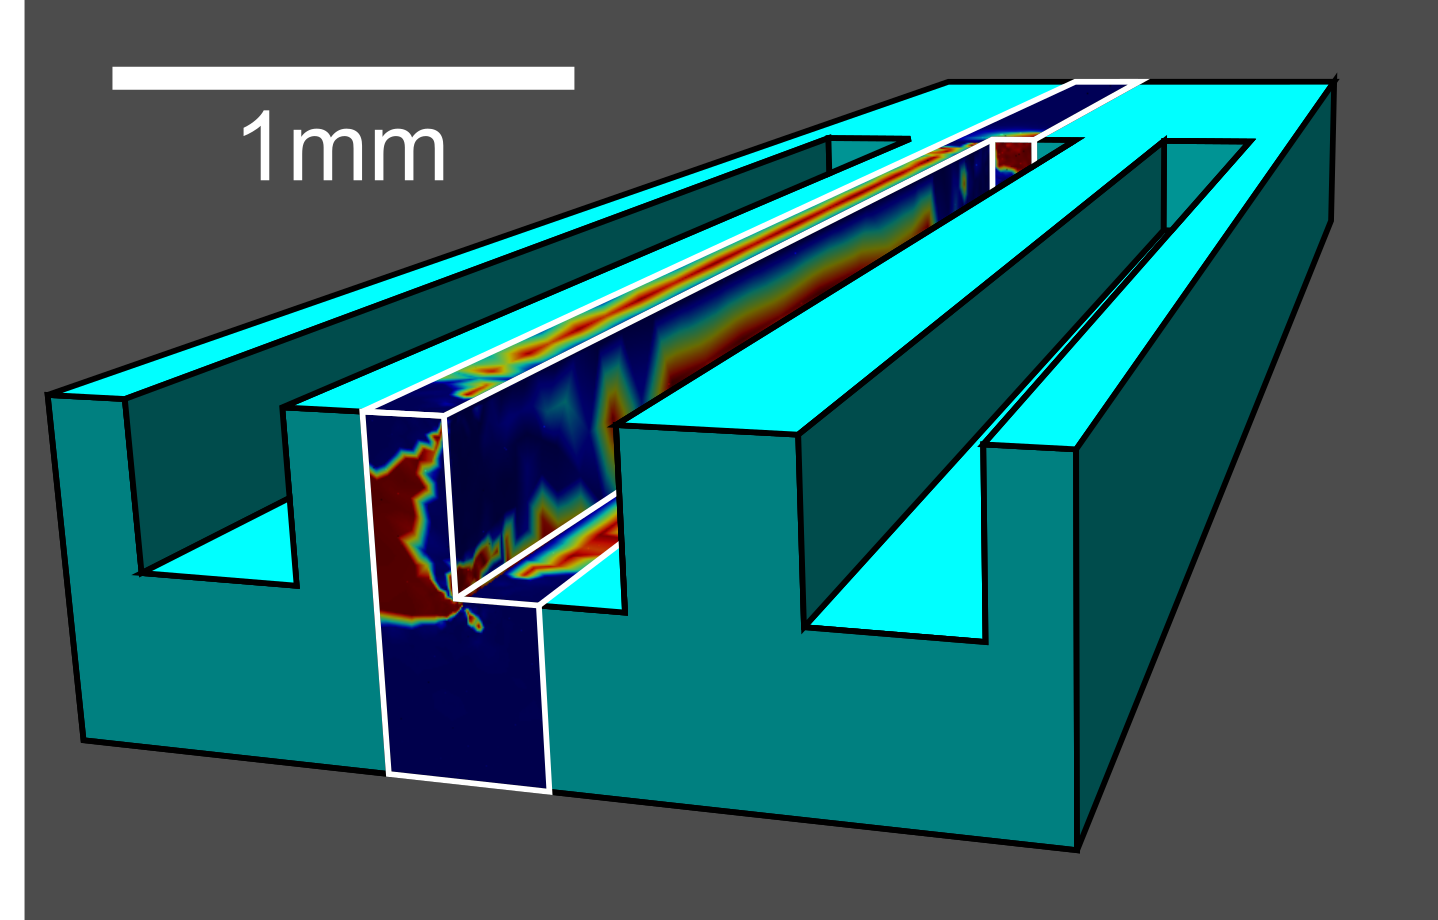
\includegraphics[width=1.0\textwidth]{figures/geometry_2D_principle.png}
\caption[2D simulation element]{To increase resolution in the critical areas, we simulate only the essential element from which by symmetry the chip can be reconstituted. The figure shows 3 groves with adjacent ridges; the minimal element being simulated comprises reaches from ridge midline to groove midline. For 2D simulations, we simulate only cells deposited as a thin layer (10$\mu\text{m}$) on top of horizontal PDMS surfaces, and the PDMS bulk. The cell culture medium, being a liquid, is considered to have negligeable mechanical influence and is not simulated. Also, surrounding portions of the culture chamber permitting interfacing with the stretch device are simulated by the boundary conditions imposed to the minimal element, but not simulated themselves. The simulated element is outlined with white edges and colors typical for simulation output, the PDMS part is cyan. The scale refers to the front plane (the grooves have a section of 350$\mu\text{m}\times350\mu\text{m}.)$}
\label{fig_2D_geometry}
}
\end{figure}

\begin{figure}
\center{
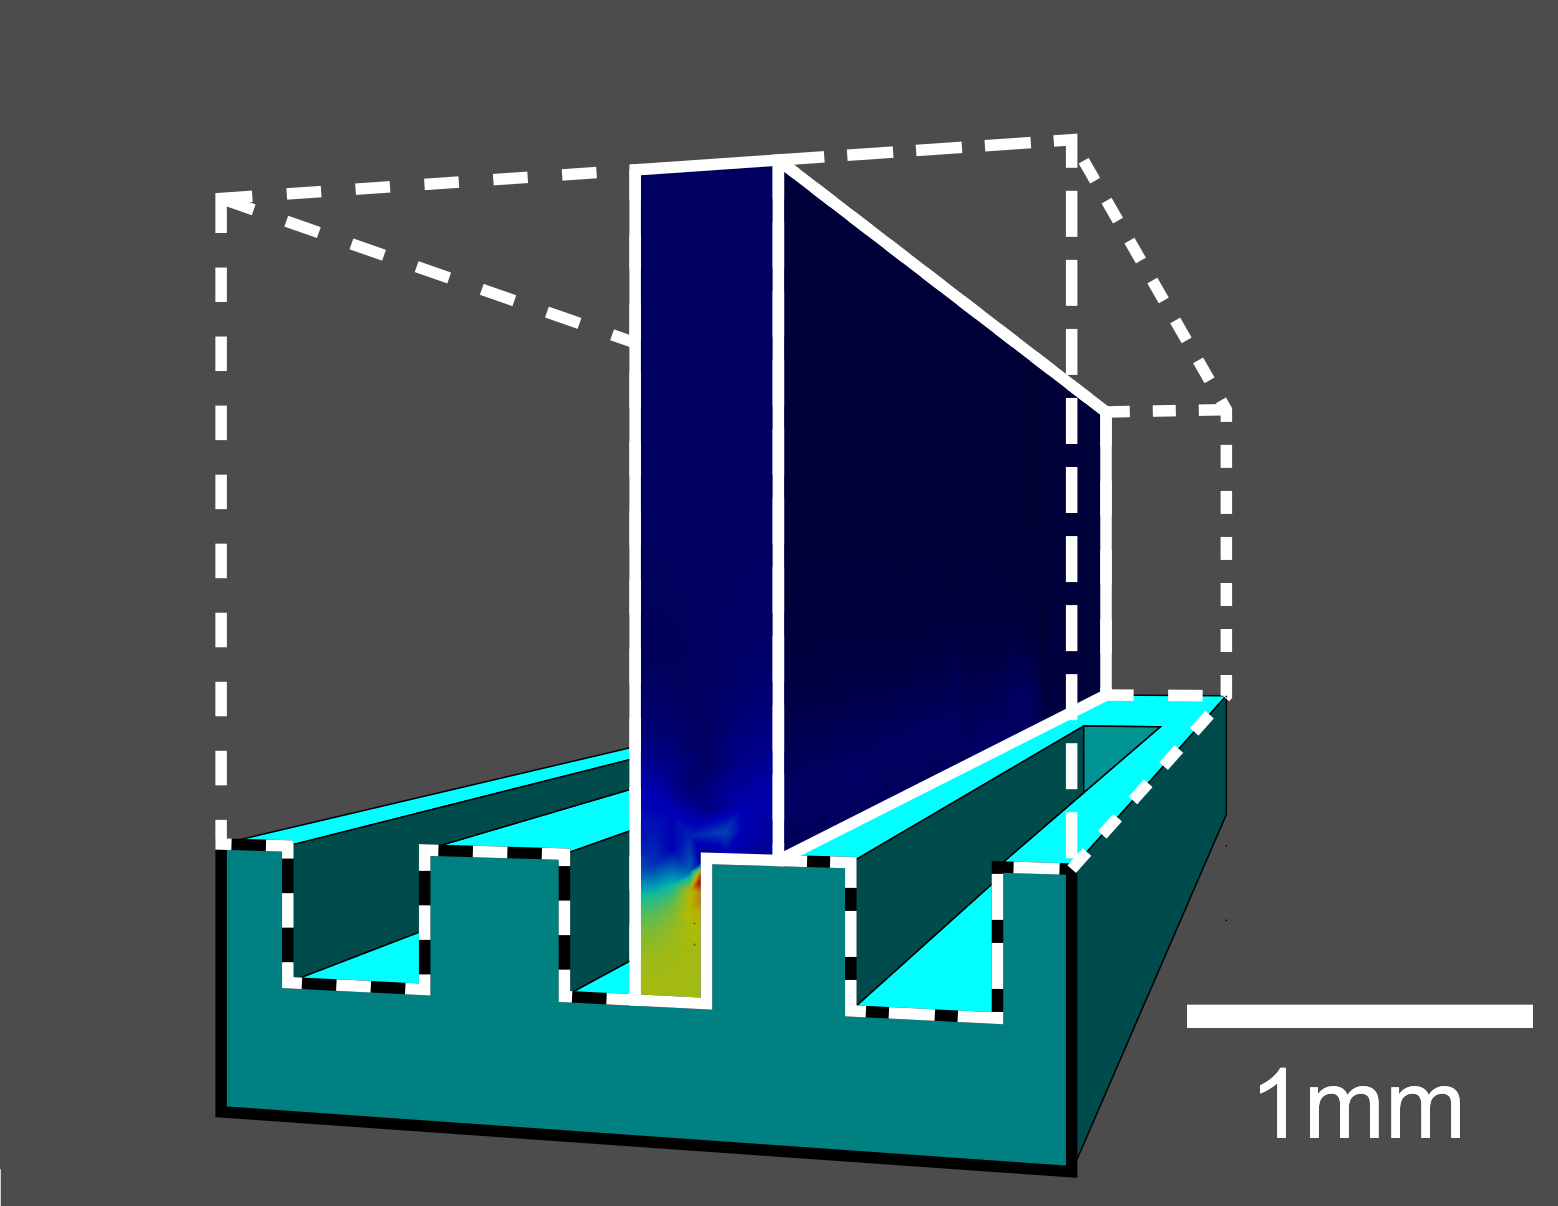
\includegraphics[width=1.0\textwidth]{figures/geometry_3D_principle.png}
\caption[3D simulation element]{The figure shows a simulation element (in heatmap colors) for 3D simulation. Only the hydrogel part is considered (white edges, drawn out for the simulated part, dashed for the remainder of the hydrogel). The PDMS imposes boundary conditions of extension but is not simulated per se. The scale refers to the front plane (the grooves have a section of 350$\mu\text{m}\times350\mu\text{m}.)$}
\label{fig_3D_geometry}
}
\end{figure}

We address two scenarii:

1. Cells seeded on top of the PDMS structures. In this case, the cells are modelled as a thin layer, no hydrogel is present. The minimal element simulated with symmetry conditions is shown in Fig. \ref{fig_2D_geometry}.


2. Cells seeded homogeneously throughout a volume of hydrogel deposited on the PDMS structure. In this case, we focus simulation on the hydrogel, and do not include the PDMS explicitly, only through extension of the hydrogel structure via the boundary conditions.  This is shown in Fig. \ref{fig_3D_geometry}.


The boundary conditions used are more trivial in some cases than in others. Free surfaces (in contact with cell culture liquid but no other material, nor part of symmetry planes) were left free. In these cases, no supplementary linear or bilinear terms arise. In both "2D" and "3D" simulations we fix the simulation in space by imposing displacement components of $u_x=0$, $u_y=0$ and $u_z=0$ on boundary faces in the vicinity of the origin, which is chosen to the right, lower corner towards the viewer in figures \ref{fig_3D_geometry} and \ref{fig_3D_geometry}. There are three such faces ($xy$, $yz$, $xz$). We aim at having for each of these three faces the corresponding normal displacement at 0: $u_x=0$ for the $yz$ face near the origin, $u_y=0$ for the $xz$ face and $u_z=0$ on the $xy$ face. These boundary conditions are thus not proper Dirichlet conditions since only one, but not all components should be tied to zero, and we use the penalty mechanism\cite{babuska_finite_1973} for achieving near Dirichlet boundary conditions for the component of interest, using eq. \ref{eq_B_penalty} and eq. \ref{eq_A_penalty}, restricted to the particular normal component of interest. Since the target displacement is zero, only the linear form (eq. \ref{eq_B_penalty}) contributes in this particular case.  

In case of the hydrogel, contact surfaces with the PDMS were also modelled through the penalty mechanism, amounting to partial flexibility with a spring equivalent (Robin boundary condition\cite{gustafson_third_1998}); this emulates the experimentally observed partial adhesion and partial detachment on these faces. For the 3D simulations where external stretch was applied, we used a linearly increase displacement target in the bilinear form. For example, for a relative chip extension $\gamma$ in the $x$-direction, we would set $u_{\text{target, }x}=\gamma \cdot x$ in eq. \ref{eq_A_penalty} in addition to using eq. \ref{eq_B_penalty}. This approximates flexible force transmission from the PDMS with to the hydrogel without actual simulation of the PDMS itself. For the 2D simulations, stretch was on the contrary imposed as fixed displacement on the appropriate end surfaces, depending on stretch direction. For the vertical symmetry planes not fixed to the origin, either displacement was imposed if stretch was applied through it, or it was imposed to be vertical (normal displacement constant) in the absence of net force when no stretch was applied through them. To satisfy this last condition, the constant displacement was optimized such that zero net force would be transmitted through these symmetry faces.

\section{Results}

\subsection{Cyclic mechanical stimulation}

This section describes the simulation results regarding external mechanical deformation of the structures. In this section, this is considered in isolation, the action of cells being considered later.

Based on the concept of strain avoidance, and particularly compressive strain avoidance, the primary active phase of the cyclic stretching should be the compression phase. Based on this reasoning, we evaluate strain field and ensuing potential cell orientation for simple chip compression. This simplification is well applicable in the $xy$-plane where compression of the entire device is indeed expected to mostly lead to compressive local strains. In the $z$-direction, due to compensatory deformation due to non-zero Poisson coefficients, high compressive strains are rather observed during device extension. Since, according to image analysis, our main focus lies on evaluation in the $xy$-plane, we restrict here analysis of cell orientation to $xy$-plane and limit the analysis to the maximum compression part of the cycle.

\subsubsection{Deformation field}


\begin{figure}
\center{
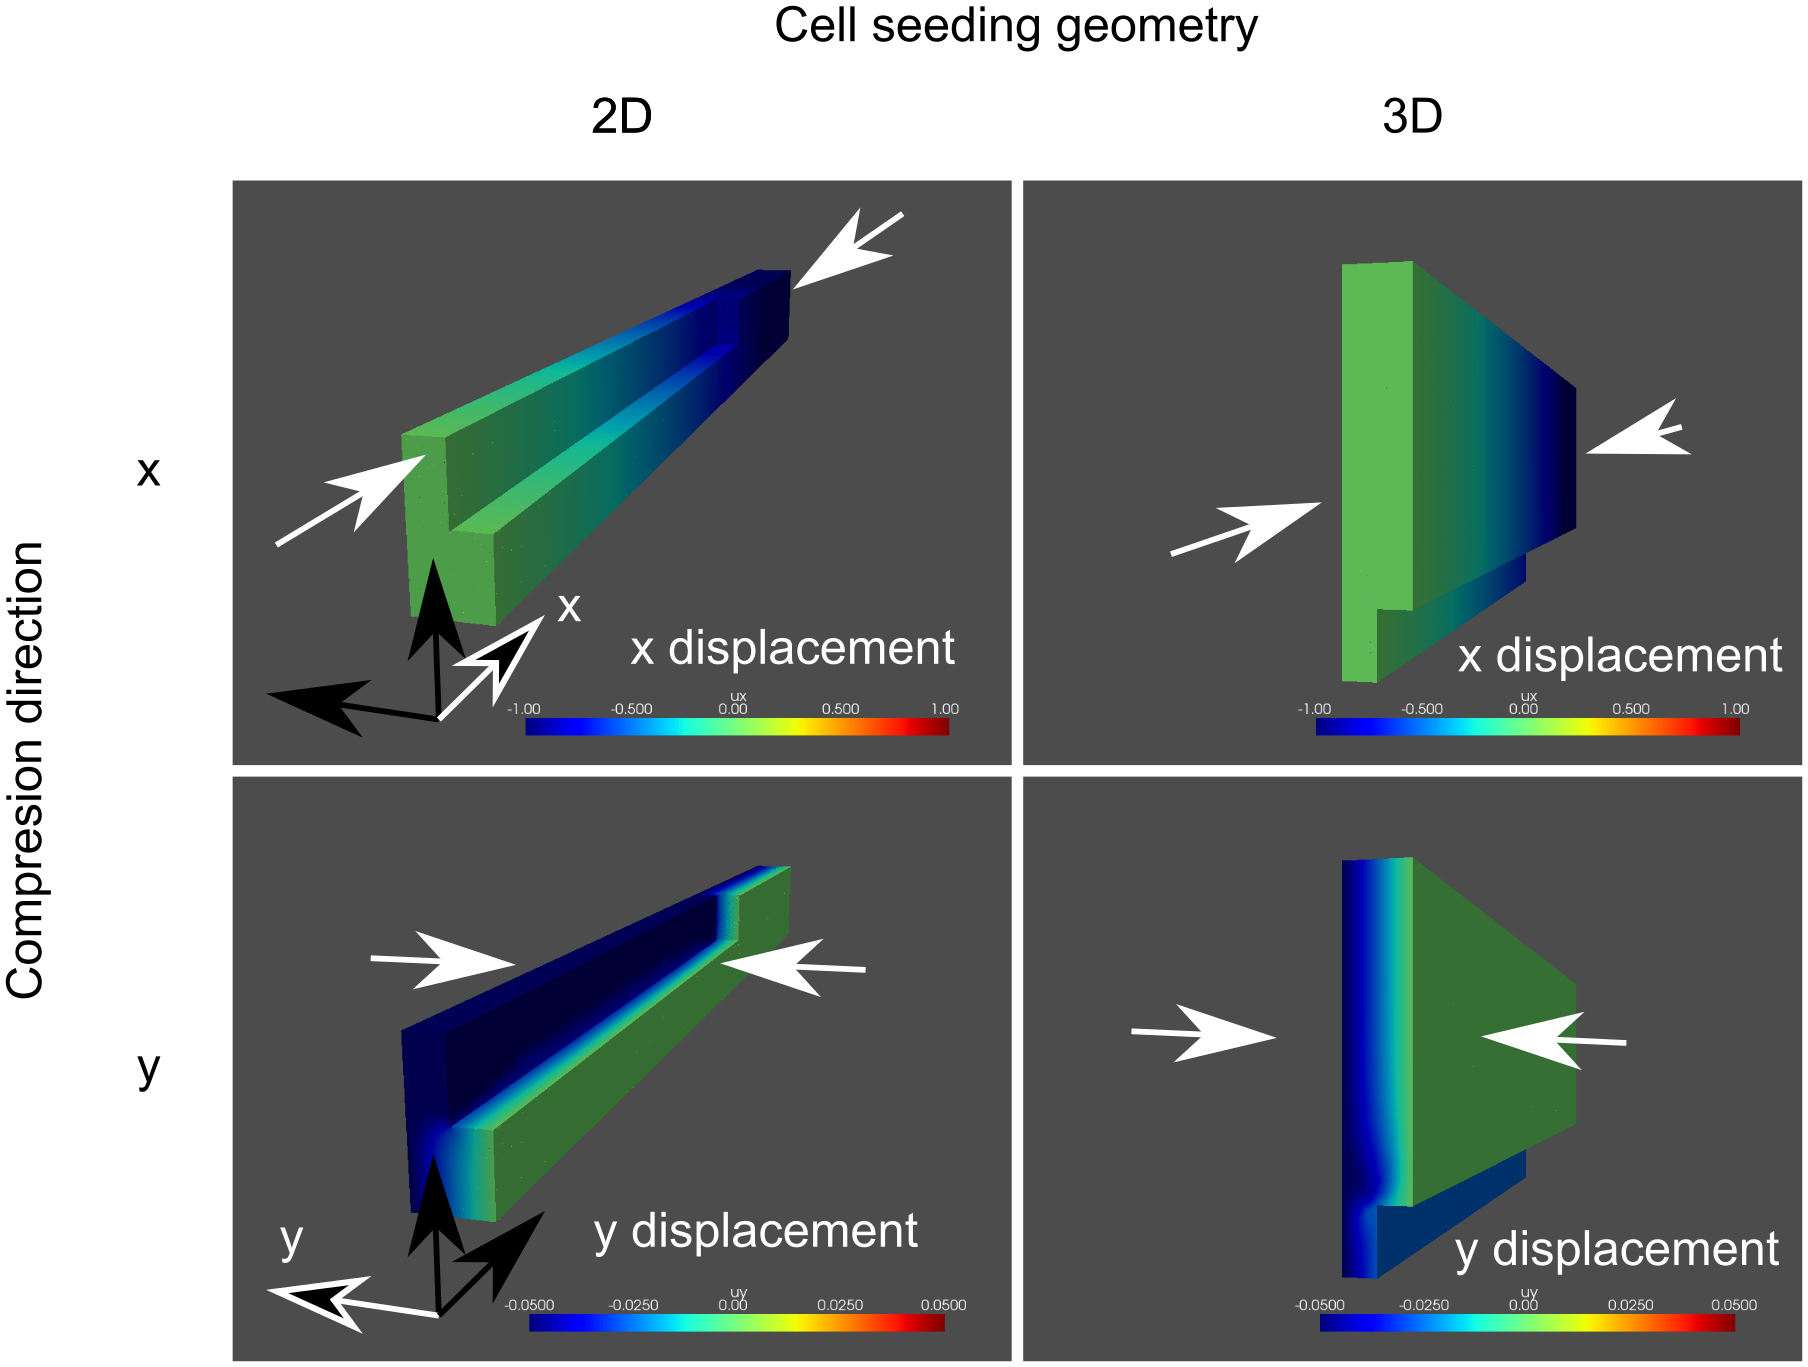
\includegraphics[width=1.0\textwidth]{figures/figure_3_deformation_field.png}
\caption[Deformation field]{Deformation in the main direction of interest for the "2D" and "3D" cell seeding geometries.}
\label{fig_deformation_field}
}
\end{figure}

Fig. \ref{fig_deformation_field} shows the main component of interest of the deformation field in different configurations. In the case of compression along the $x$-axis, which is along the grooves, the main compression component of interest shown here is the $x$ component of the displacement field, in the case of compression along the $y$-direction, the $y$-component of the displacement field is shown. In both the "2D" geometry (where cells are assumed to be seeded on top of the structures) and the "3D" geometry, where cells are assumed to be seeded throughout the hydrogel slab volume, one can see that the externally imposed compression translates to the anticipated gradient in deformation aligned with the direction of compression.


\begin{figure}
\center{
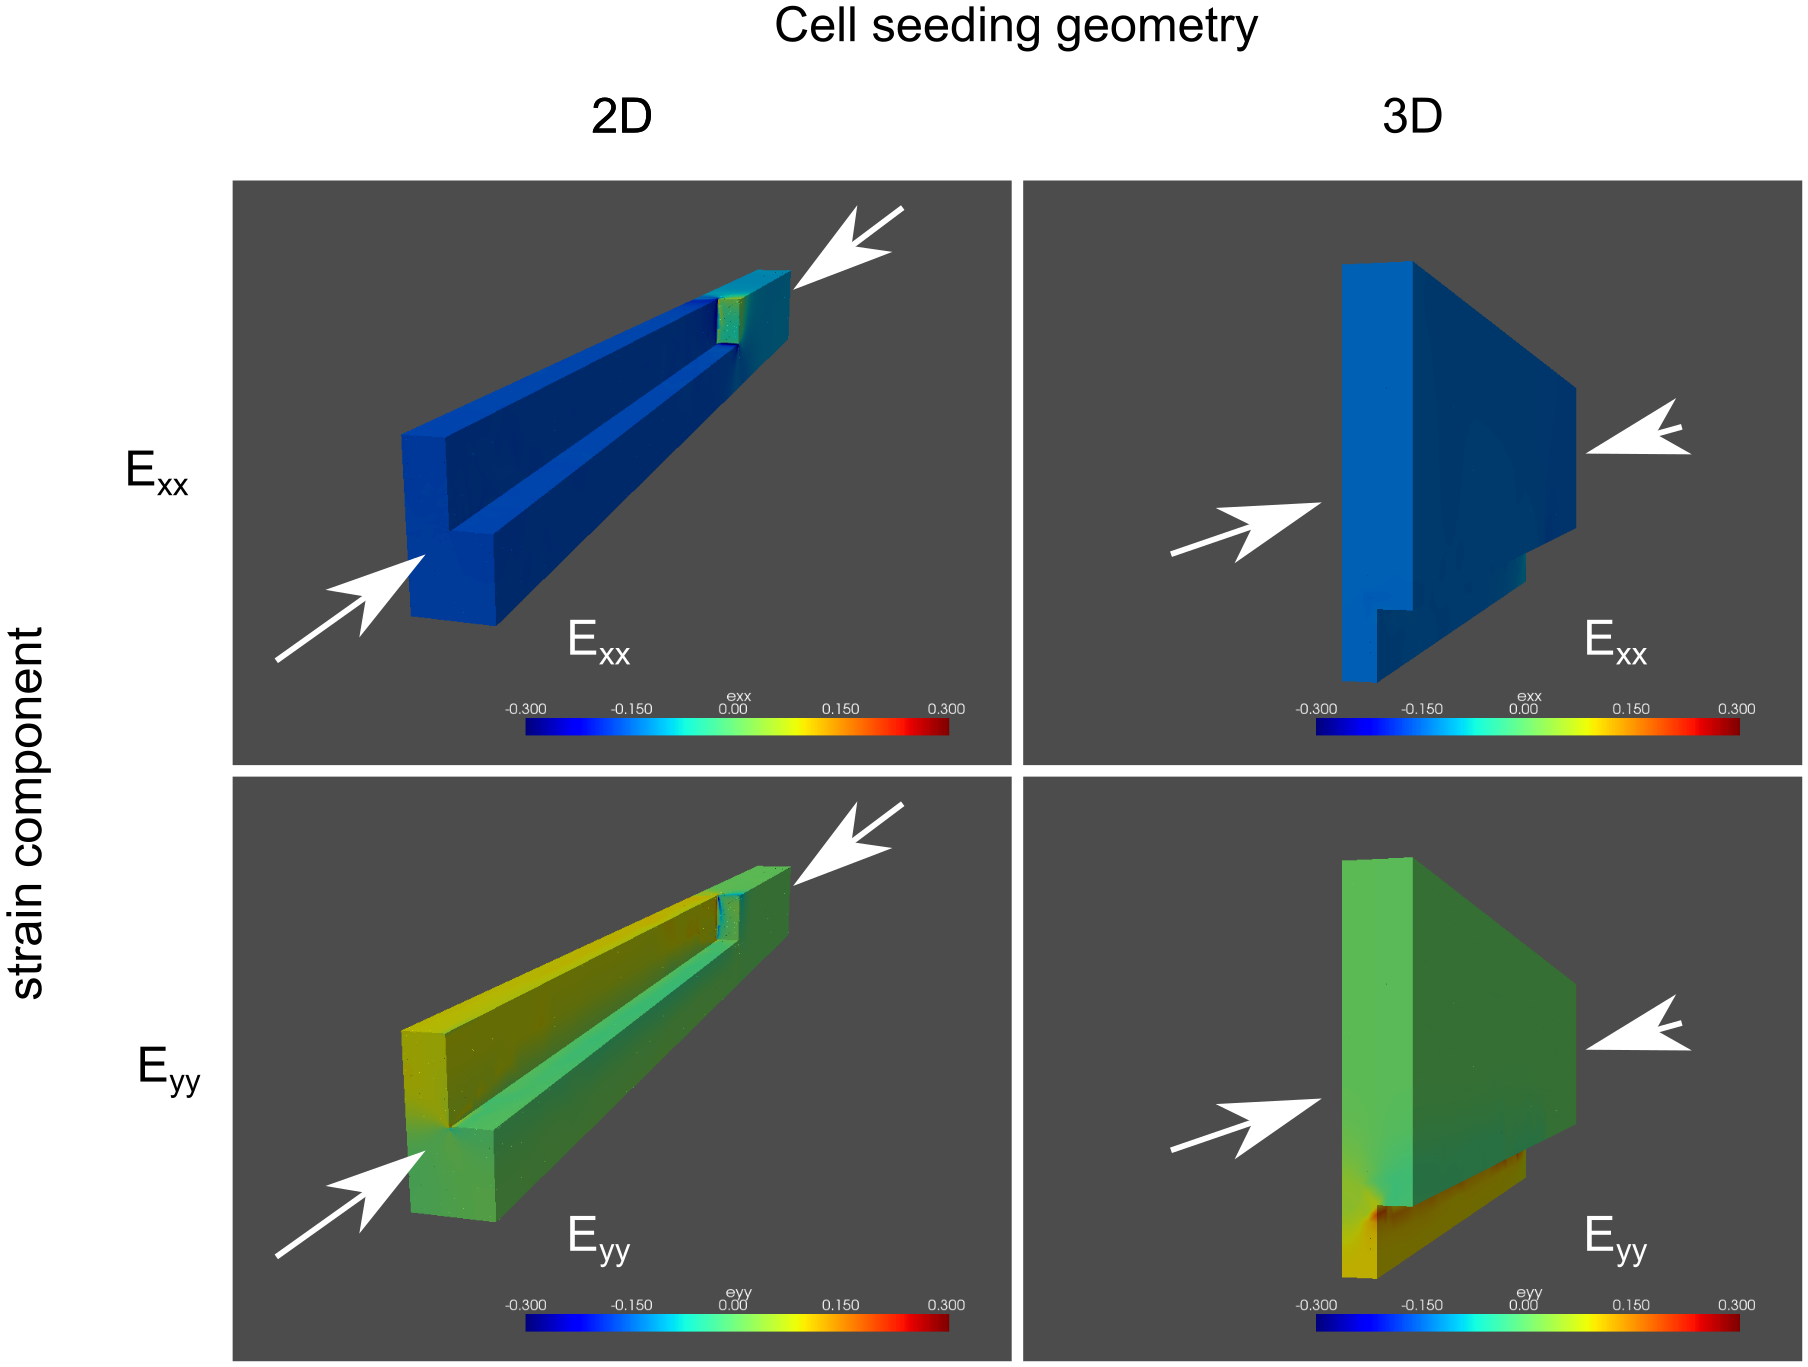
\includegraphics[width=1.0\textwidth]{figures/figure_4_strain_field_along.png}
\caption[Strain field compression along grooves]{Main strain components in the $xy$-plane for compression along the grooves during cyclic stretch. Simulation with 30\% external stretch applied, for both "2D" and "3D" cell seeding geometries.}
\label{fig_strain_field_along}
}
\end{figure}

\subsubsection{Strain field}




Fig. \ref{fig_strain_field_along} shows the main in-plane strain components, that is $\epsilon_{xx}$ and $\epsilon_{yy}$ for compression of the chips along the direction of the grooves. One can see similar resulting patterns for both the 2D cell seeding geometry (PDMS+thin cell layer, c.f. Fig. \ref{fig_2D_geometry}) and the 3D cell seeding geometry (simulation of the hydrogel slab only, c.f. Fig. \ref{fig_3D_geometry}). Indeed, in both cases, a negative (compressive) strain results along the direction of compression as expressed by substantially negative values of $\epsilon_{xx}$, as one would anticipate, whereas in the perpendicular direction the $\epsilon_{yy}$ values remain closer to 0. 



\begin{figure}
\center{
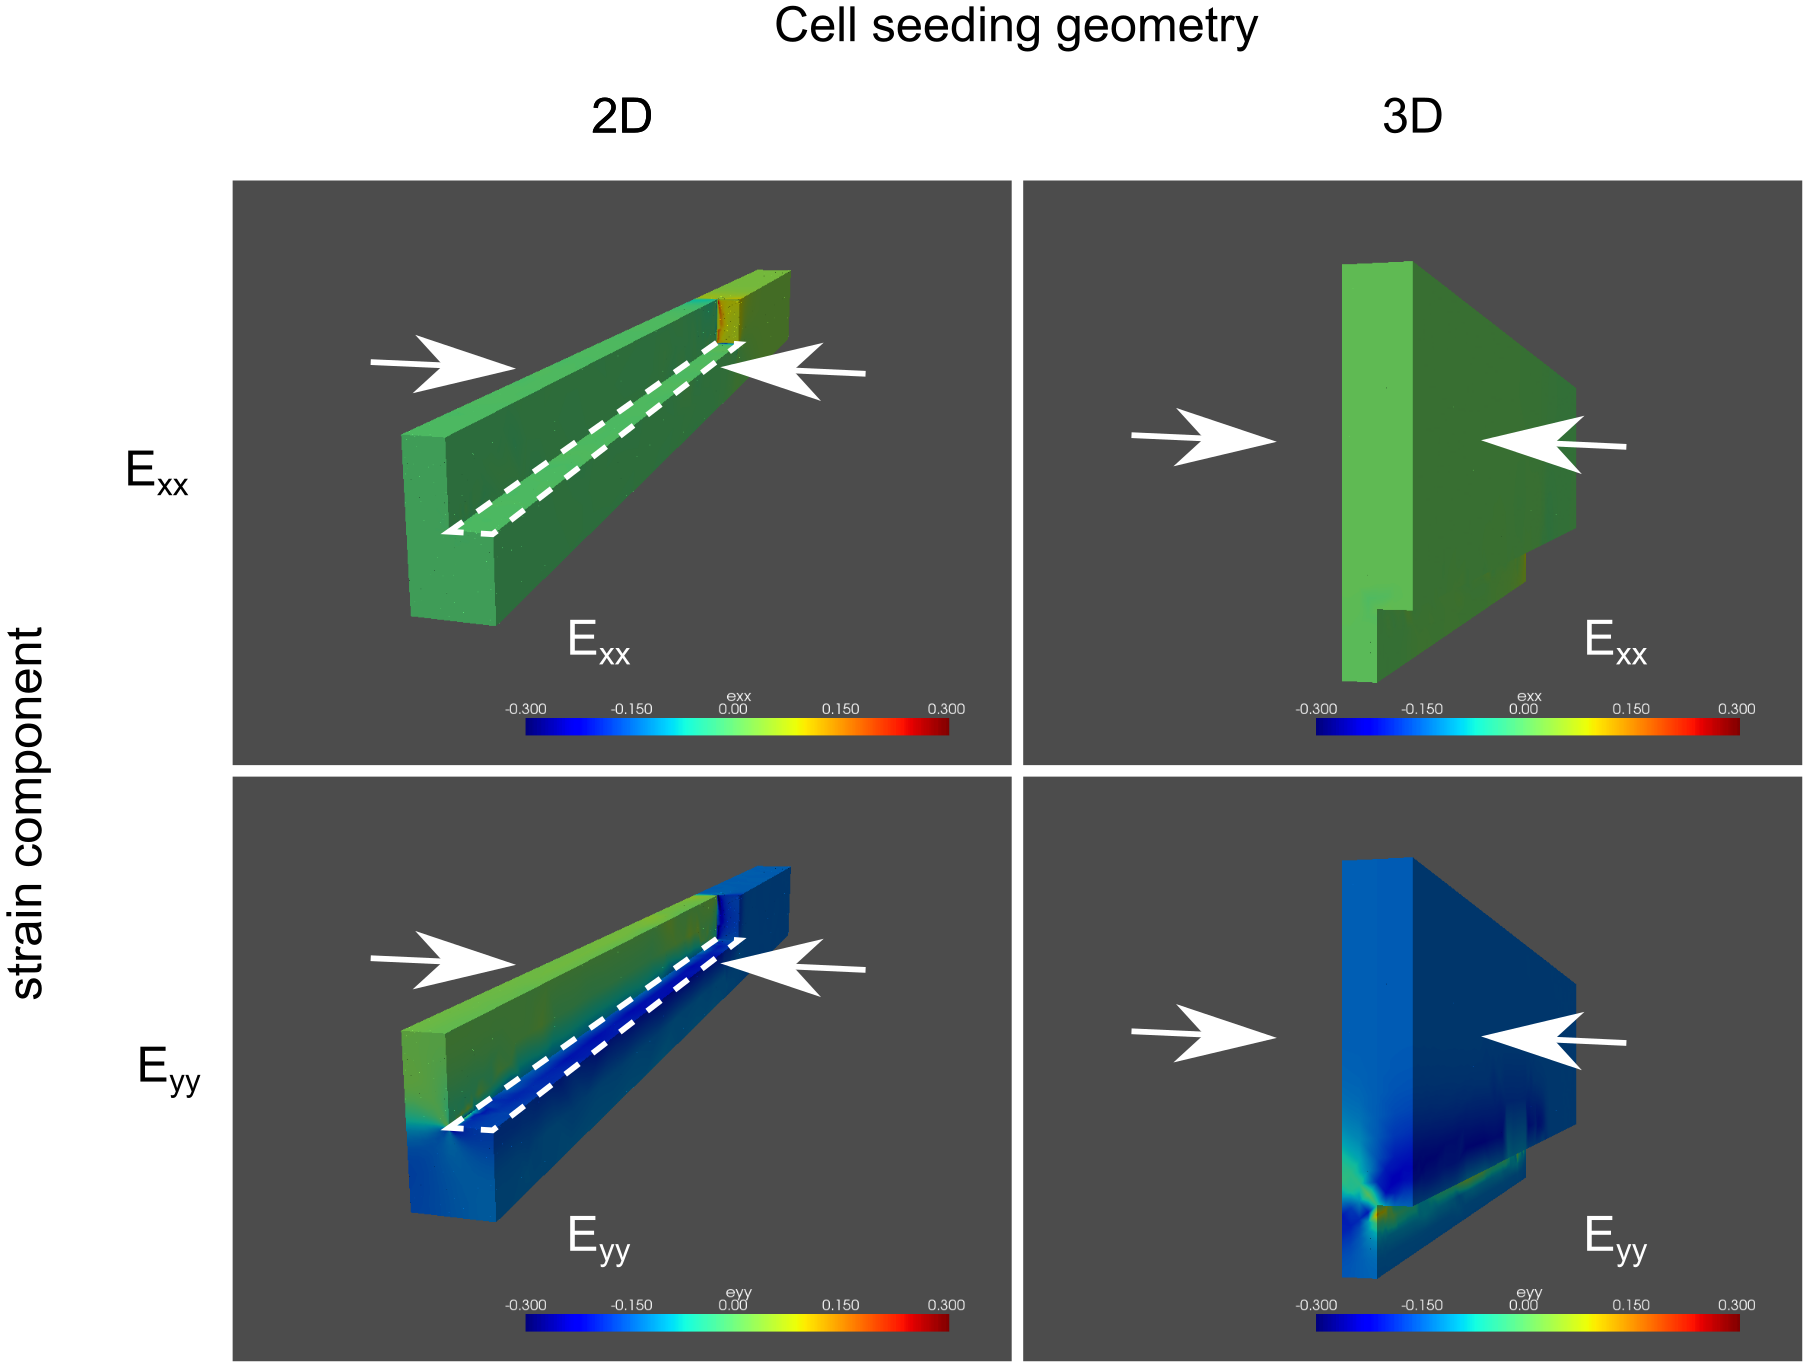
\includegraphics[width=1.0\textwidth]{figures/figure_5_strain_perpendicular.png}
\caption[Strain field compression perpendicular to grooves]{Main strain components in the $xy$-plane for compression along the grooves during cyclic stretch. Simulation with 30\% external stretch applied, for both "2D" and "3D" cell seeding geometries.}
\label{fig_strain_field_perpendicular}
}
\end{figure}

Fig. \ref{fig_strain_field_perpendicular} shows the main in-plane strain components $\epsilon_{xx}$ and $\epsilon_{yy}$ for compression of the chips perpendicularly to the direction of the grooves. Again, the patterns are globally similar between "2D" and "3D" cell seeding geometries, with an important compressive component this time in the $y$ direction, materialized by negative $\epsilon_{yy}$ values. Of note, in the case of the "2D" geometry, the ridge experiences only very partial compression, effective deformation is limited to the bottom of the channel, outlined with a white dashed line. This is typically also the primary zone of interest in imaging from below due to the shortest working distances.

\subsubsection{Cell orientation}

\begin{figure}
\center{
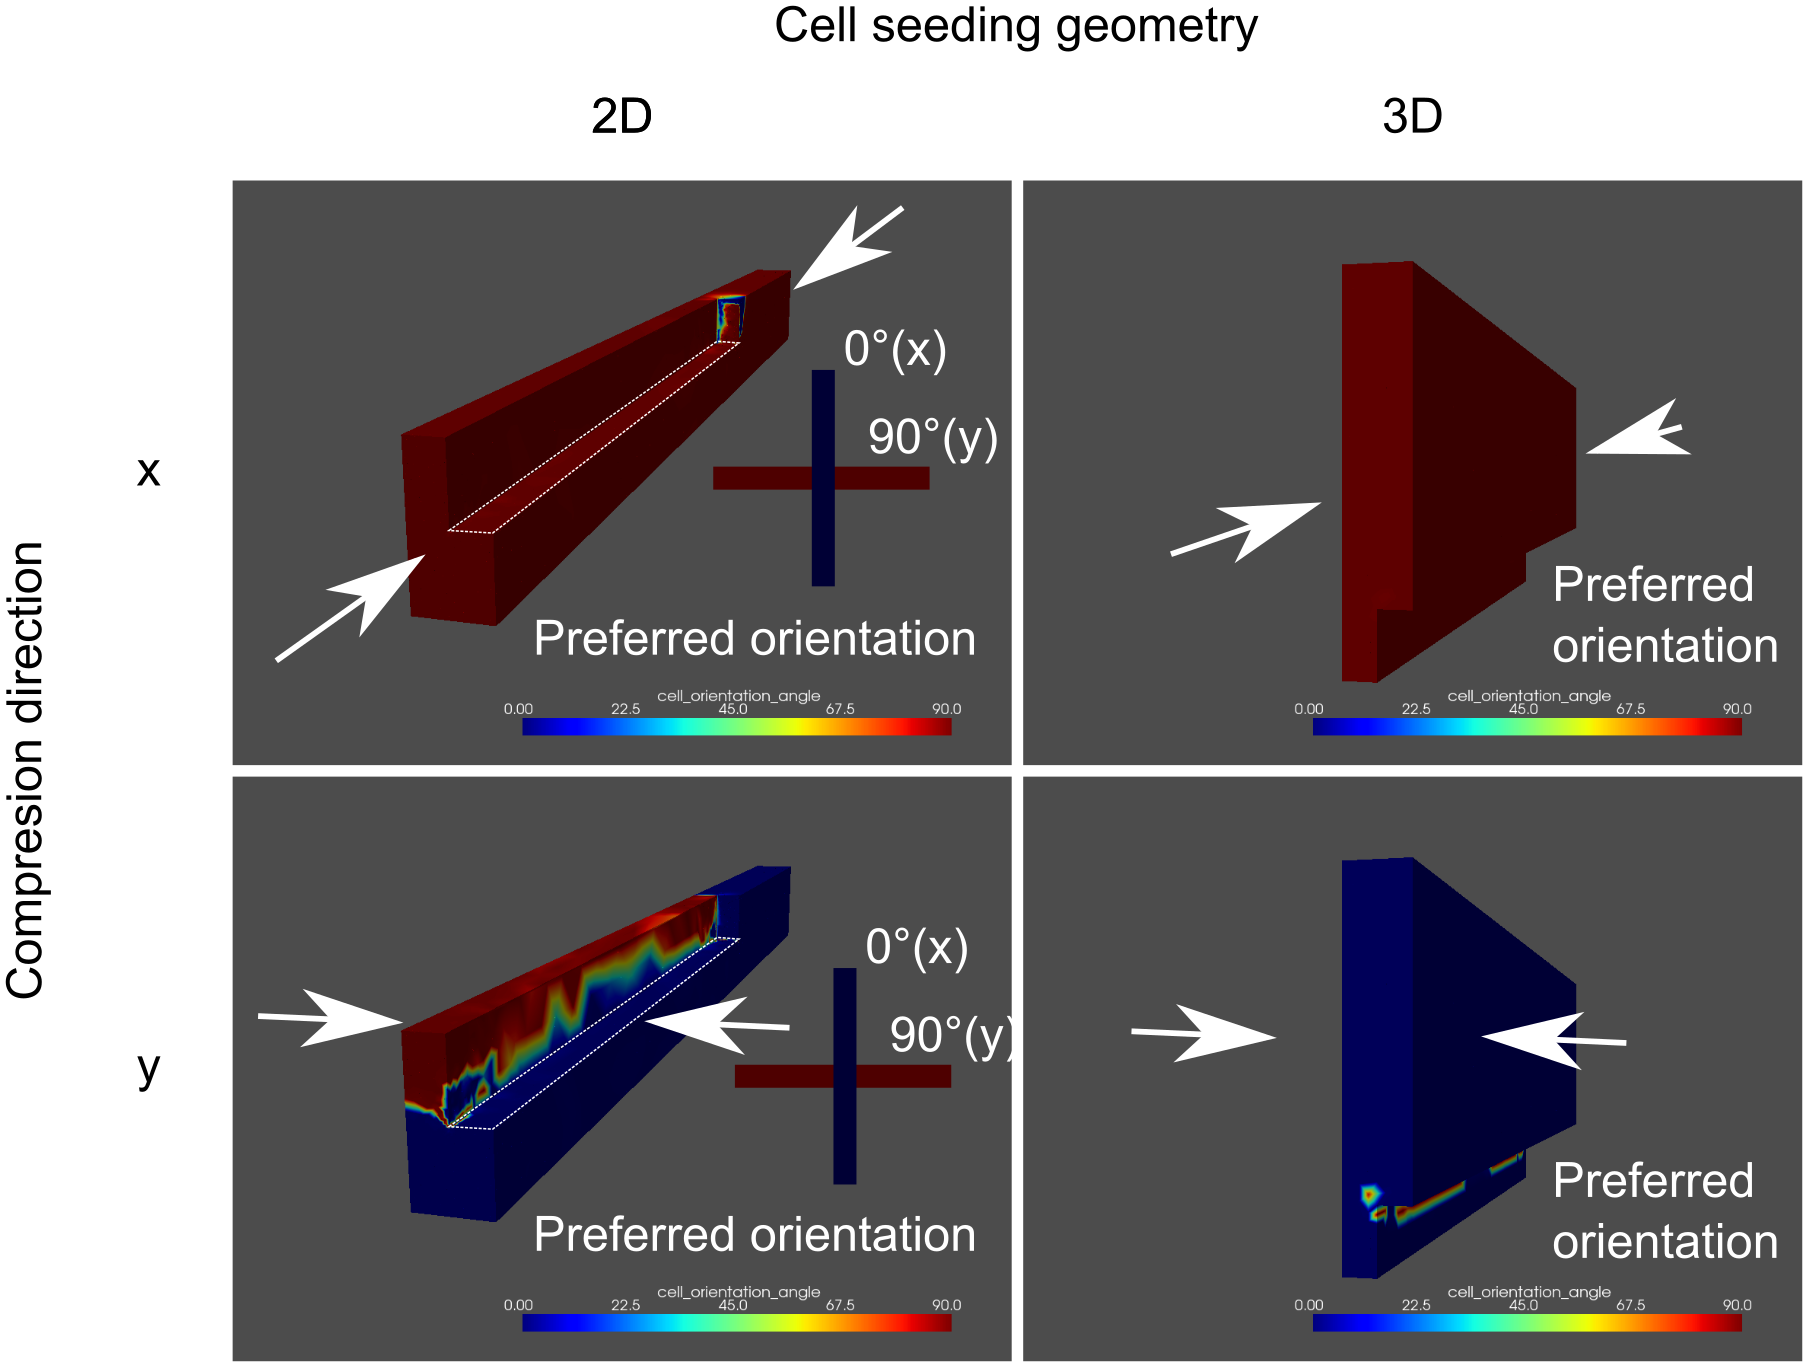
\includegraphics[width=1.0\textwidth]{figures/figure_6_cell_orientation.png}
\caption[Cell orientation]{Potential cell orientation evaluated as the least compressive eigen vector direction in the $xy$-plane, for "2D" and "3D" cell seeding geometries and externally applied compression along the grooves (top row) and perpendicular to the grooves (bottom row).}
\label{fig_cell_orientation_single_effect}
}
\end{figure}

From the strain analysis (Fig. \ref{fig_strain_field_along} for compression along the grooves and Fig. \ref{fig_strain_field_perpendicular} for compression applied perpendicularly to the grooves), one can evaluate a preferred cell orientation. For this, we use the full set of in-plane strains (thus, $\epsilon_{xx}$, $\epsilon_{xy}=\epsilon_{yx}$ and $\epsilon_{yy}$) to derive the directions associated with the highest and lowest compressive strain as the direction associated with the highest and lowest eigenvalue of the strain matrix. Strain avoidance then would predict the least compressive direction to give the preferred direction for cell alignment, at least to within the extent of the relative naive lumped cell orientation model used here.

Figure \ref{fig_cell_orientation_single_effect} shows the predicted cell orientations for the scenarii of 2D seeding on top of the PDMS structures and 3D seeding with a hydrogel slab. Cyclic stretch along the grooves is predicted to uniformly favor cell orientation perpendicular to the grooves (90° in Fig. \ref{fig_cell_orientation_single_effect}), whereas cyclic stretch perpendicularly to the grooves favours cell orientation along the grooves, although there are additional effects at play for this scenario. Particularly in the "2D" scenario, deformation is only incompletely transmitted to the ridges through their base (c.f. Fig. \ref{fig_strain_field_perpendicular}), whereas compensatory effects due to the nearly incompressible nature of the PDMS cause additional strain to appear. As a result, the preferred cell orientation on the ridges is less well defined and more variable. To some extent, stress concentration effects near the edges have a similar effect in the 3D scenario (see Fig. \ref{fig_strain_field_perpendicular}).

Beyond the primary preferred orientation, as given in Fig. \ref{fig_cell_orientation_single_effect} for different scenarii, one can also wonder about the strength of the orientation imparted. For this, we define the stretch ratio as:

\begin{equation}
r=\frac{1+\lambda_{\text{max}}}{1+\lambda_{\text{min}}} \label{eq_r}
\end{equation} 

where $\lambda_{\text{max}}$ and $\lambda_{\text{max}}$ are the maximal and minimal eigen-value of the strain matrix as restricted to the $xy$-plane. Indeed, $r$ as defined by eq. \ref{eq_r} is 1 in the absence of deformation ($\lambda_{\text{max}}=\lambda_{\text{min}}=0$) and remains 1 in the case of isotropic deformation for which $\lambda_{\text{max}}=\lambda_{\text{min}}$ holds.

\begin{figure}
\center{
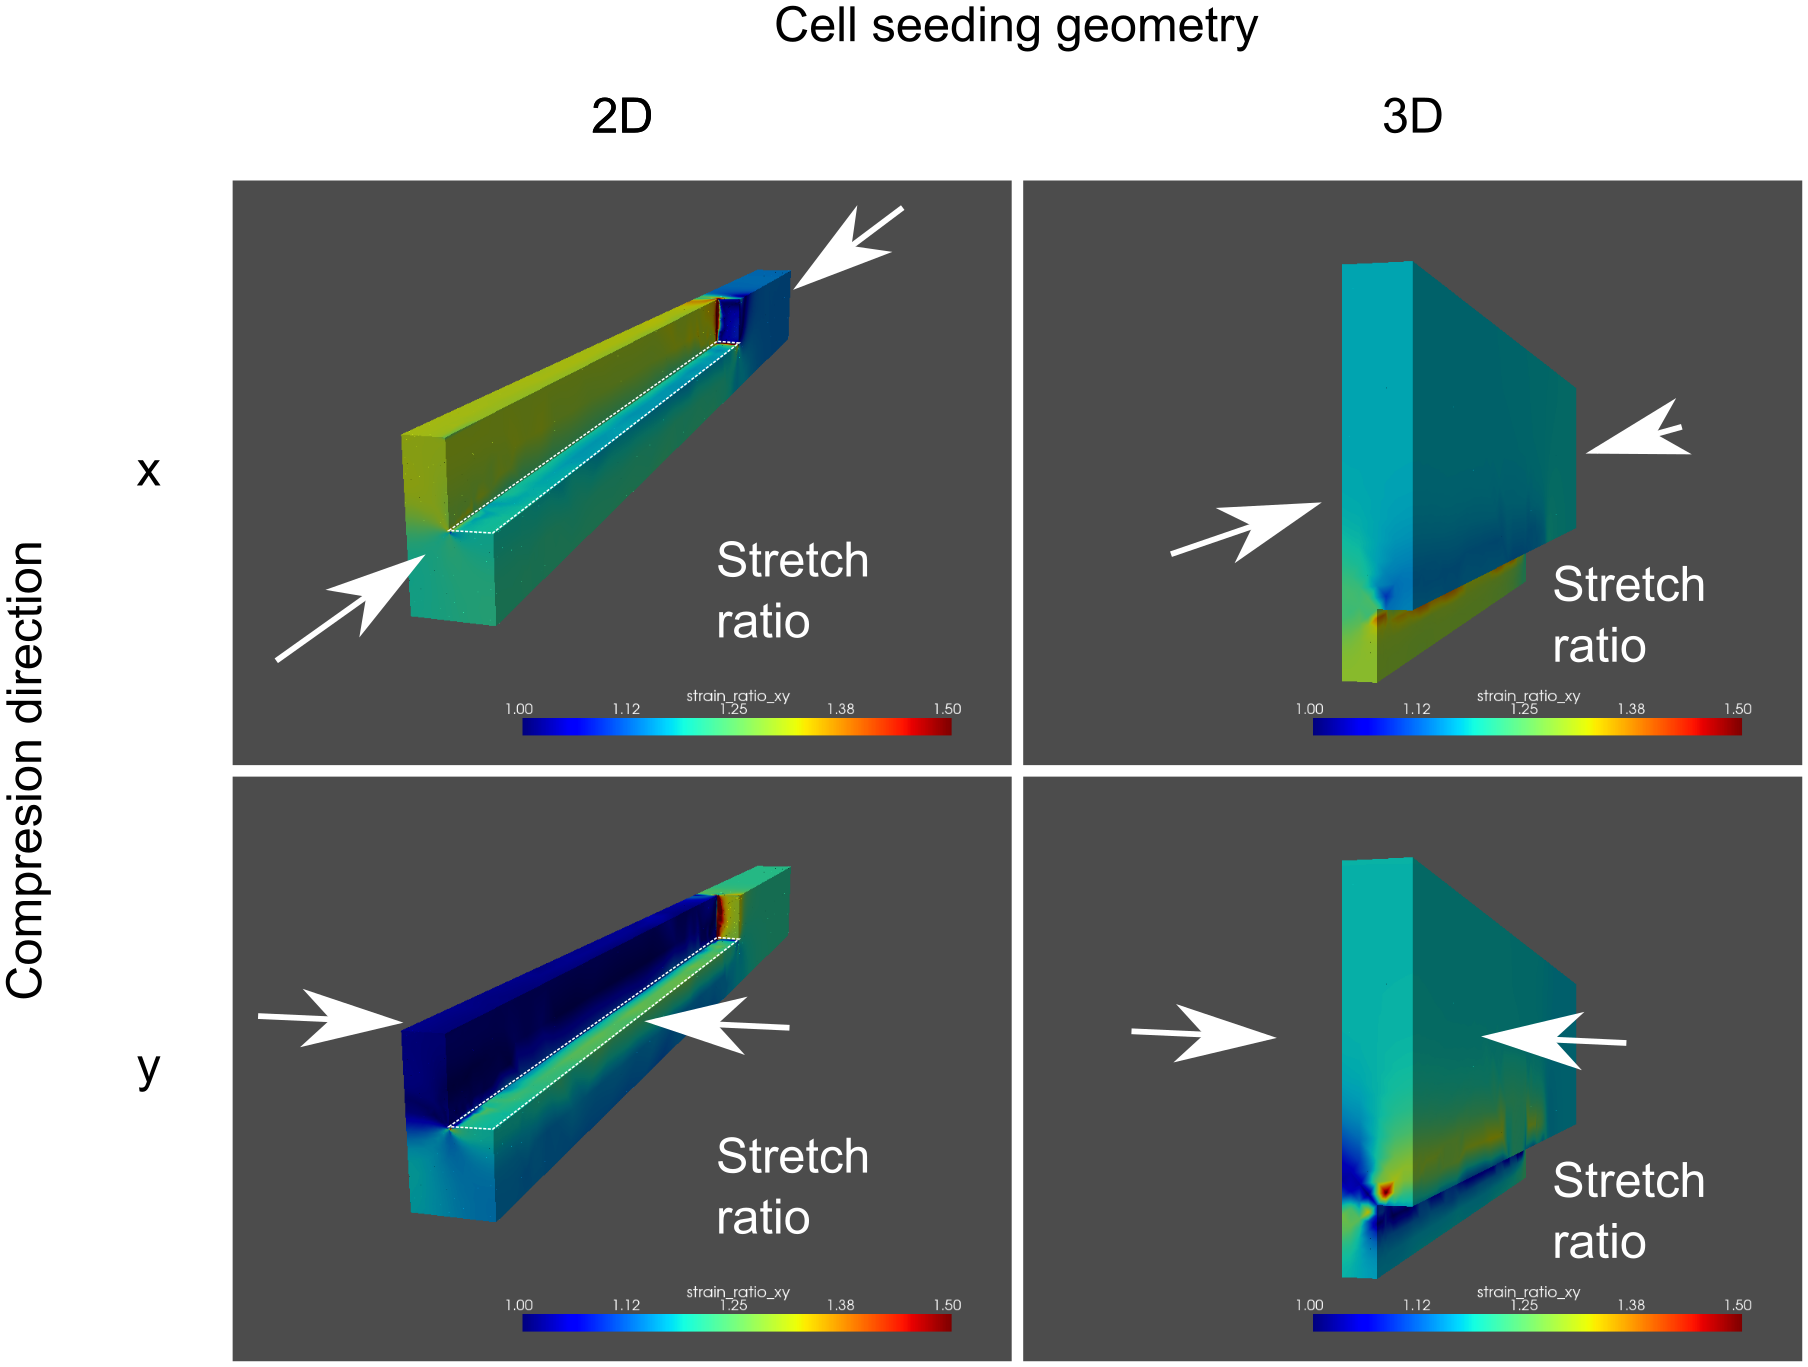
\includegraphics[width=1.0\textwidth]{figures/figure_7_stretch_ratio.png}
\caption[Stretch Anisotropy]{Stretch ratio according to eq. \ref{eq_r} as a measure of local anistropic deformation. A stretch ratio close to 1 indicates little effect on cell orientation, whereas larger stretch ratios predict strong influence on cell orientation.}
\label{fig_stretch_ratio}
}
\end{figure}

Fig. \ref{fig_stretch_ratio} shows the stretch ratio as defined by eq. \ref{eq_r} for the 2D and 3D cell seeding cases, in scenarii with mechanical stimulation applied along and perpendicularly to the grooves. Comparing Fig. \ref{fig_stretch_ratio} and fig. \ref{fig_cell_orientation_single_effect}, it can be seen that the relatively uniform cell orientation predicted when stretching along the grooves is assorted with a relatively homogeneous stretch ratio distribution, with important strain inhomogeneity everywhere. In the case of mechanical stretching perpendicular to the grooves, it can be seen that regions with a stretch ratio closer to 1 occur.They coincide with the regions where cellular orientation perpendicular to the grooves was predicted. Thus, we are lead to adjust our statement about cell orientation with mechanical stimulation applied perpendicularly to the grooves. Indeed, we can state that applying cyclic stretch perpendicularly to the grooves should be associated with widespread orientation of cells along the grooves; towards the top of the ridges in the 2D scenario and near edges in the 3D scenario, more ambiguous and weaker cell orientation could occur with more heterogeneous and more weakly defined cell orientation. 


\subsubsection{Summary}

Summarizing the results on pure cyclic mechanical stimulation, we anticipate general cellular orientation perpendicular to the direction of applied strain, although stress concentration near edges or particularly shield areas may lead to some areas with weaker and more heterogeneous cell alignment. 


\subsection{Cellular contraction}

This section describes the simulation of the effects of cellular contraction. In this section, we consider the cellular contraction leading to local strain separately from external mechanical stimulation, only in the final results section, we shall consider the combination.


\subsubsection{Deformation field}


\begin{figure}
\center{
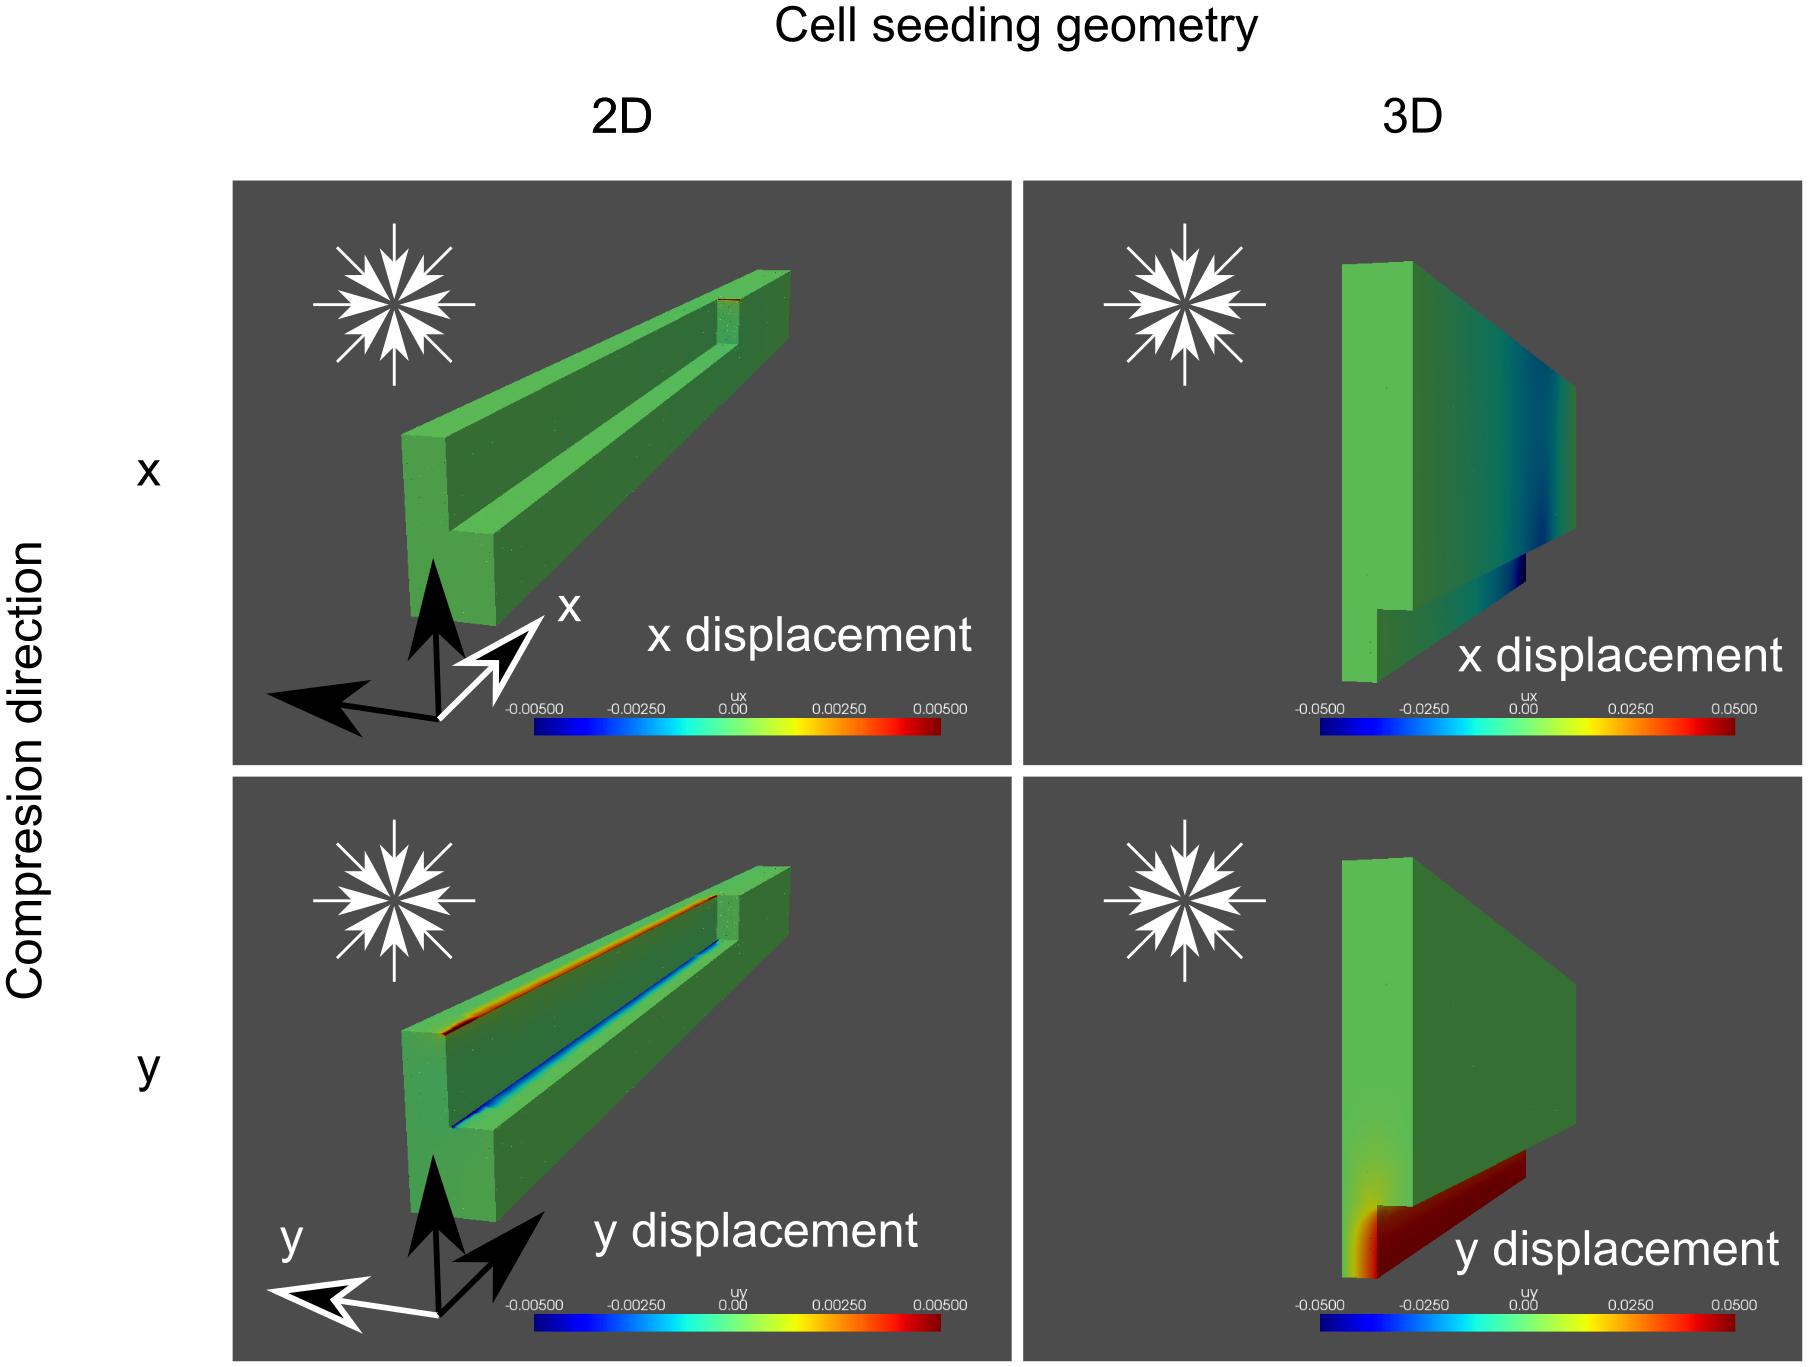
\includegraphics[width=1.0\textwidth]{figures/figure_8_deformation_field_self_condensation.png}
\caption[Deformation field]{Deformation field arising by self condensation through cellular contraction in 2D and 3D seeded geometries, $x$- and $y$-components. The equivalent free homogeneous contraction capacity is 15\% in each linear direction.}
\label{fig_deformation_field_self}
}
\end{figure}

The $x$- and $y$-components of the deformation field arising through cellular contraction are shown in Fig. \ref{fig_deformation_field_self}. Note than in the 2D geometry, the cells are assumed to present only as thin layers on the horizontal surfaces, while in the 3D geometry, they are assumed to be homogeneously distributed throughout the gel volume. Partly as a consequence of the unequal distribution, partly due to the high Young's modulus of PDMS, the amplitude of the deformations are much smaller in the 2D seeding than in 3D; indeed, the scale is different by a factor of 10, and despite that, the 3D displacements remain more visible. In addition, due to imperfect contact between the hydrogel in 3D and the PDMS (neither shown nor directly simulated, c.f. Fig. \ref{fig_3D_geometry}), the most important deformations occur in the grooves in the 3D geometry. Minor displacements in the $xy$ plane are also possible along the free edges of the colonized horizontal areas in the 2D geometry.



\subsubsection{Strain field}


\begin{figure}
\center{
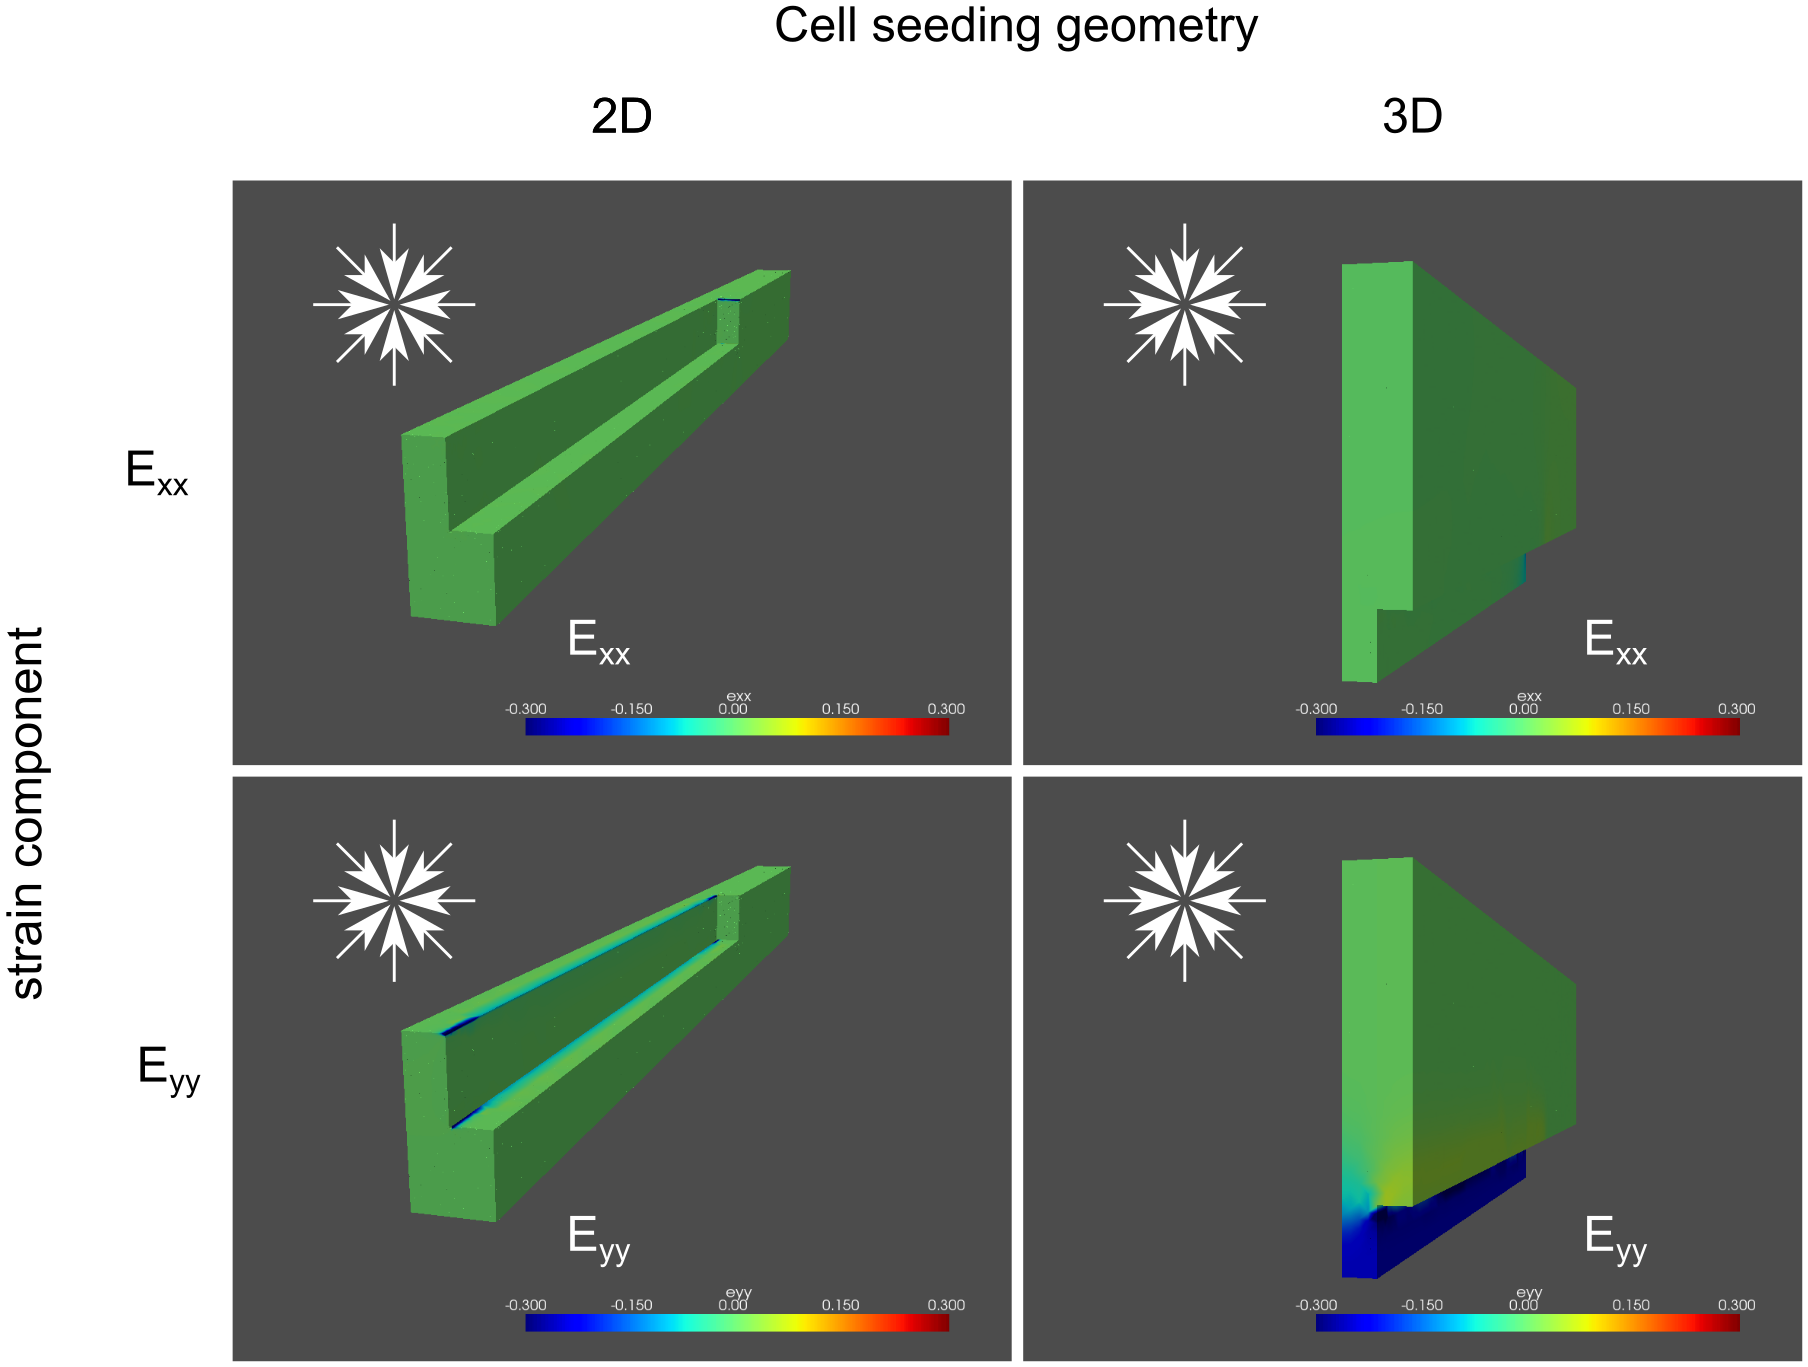
\includegraphics[width=1.0\textwidth]{figures/figure_9_strain_field_self.png}
\caption[Strain field]{Strain field arising by cellular self contraction in 2D and 3D cell seeding geometry, illustration of the main in-plane components $\epsilon_{xx}$ and $\epsilon_{yy}$. In the 2D geometry, the strain remains minor, with some contraction along the edges of the horizontal surface where cells can retract somewhat. In the 3D geometry, substantial negative (compressive) strain occurs in the $\epsilon_{yy}$ component in the grooves. }
\label{fig_strain_field_self}
}
\end{figure}

As before, we obtain the strain components from the deformation field. Fig. \ref{fig_strain_field_self} shows that the strains due cell contraction is generally very weak, and even so substantial non-zero components in the $xy$-plane are only present near the free edges of the cell lawn on the horizontal surfaces. This starkly contrasts with the strain field in the 3D hydrogel geometry. Here, strong compressive strain in the $y$ direction is present in the grooves, at a quantitative scale that can rival with the externally applied strains.


\subsubsection{Cell orientation}

\begin{figure}
\center{
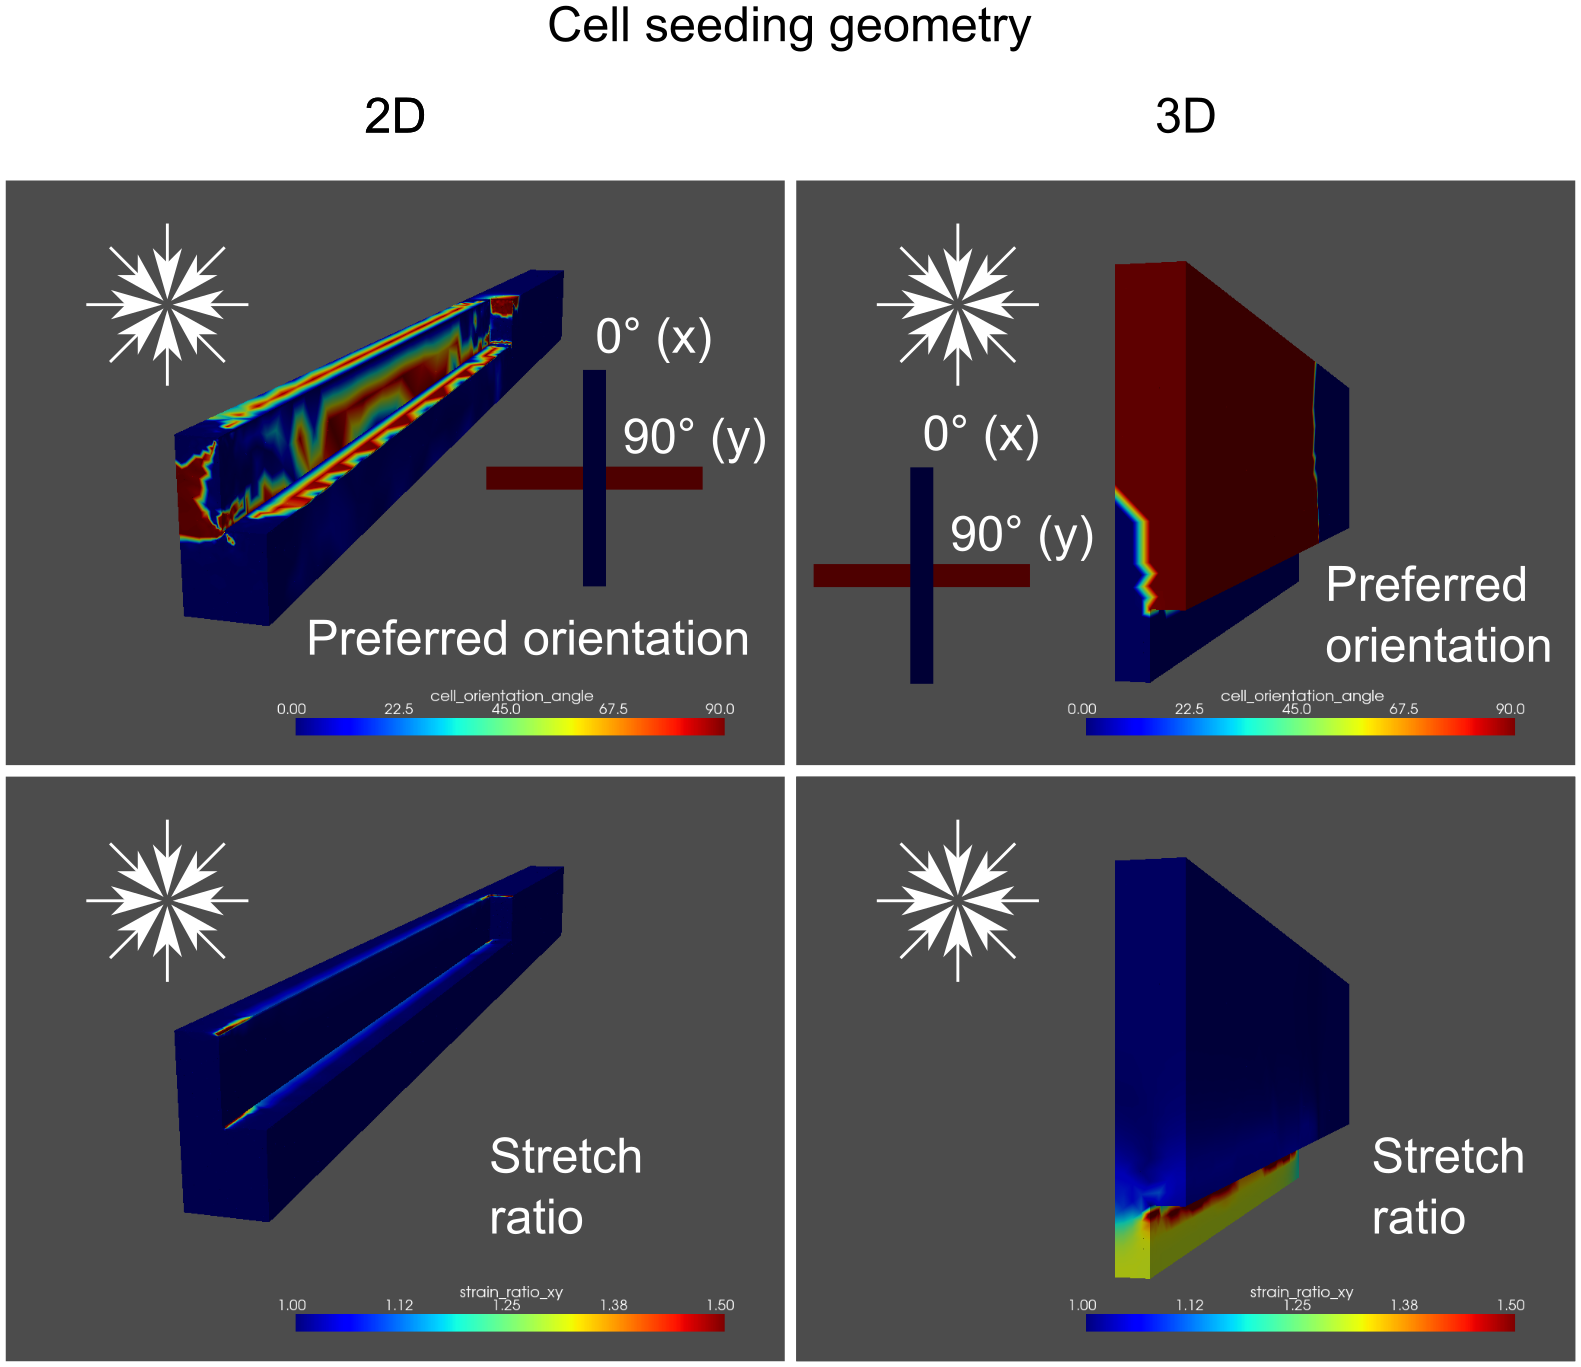
\includegraphics[width=1.0\textwidth]{figures/figure_10_cell_orientation.png}
\caption[Cell orientation]{Cell orientation potential due to self-condensation by cell contraction. The top row indicates the theoretical preferred angle along the least compressive direction in the $xy$-plane. The bottom row indicates the strength of the local strain asymmetry, via the stretch ratio calculated from eq. \ref{eq_r}}
\label{fig_cell_orientation_self_condensation}
}
\end{figure}


Fig. \ref{fig_cell_orientation_self_condensation} shows the model analysis regarding cell orientation under the sole action of self-condensation via cell contraction. In the 2D seeding configuration, the alignment effect remains weak with low local strain anisotropy (bottom left) except for in the immediate vicinity of the edges. In these areas, cell alignment along the grooves is favoured, elsewhere it is badly defined for the 2D geometry. In the 3D geometry, a strong alignment effect with strong strain anisotropy in the $xy$-plane is seen for the full volume of hydrogel occupying the grooves, but not above in the bulk hydrogel, where the alignment angle is badly defined in the presence of a stretch ratio close to 1.

The reason for the low strain values in the 2D geometry and thus mostly low strain anisotropy is the relatively high stiffness of PDMS as compared to cells. The compressive force generated by the cells thus translates only into minor deformation and thus small strain values. In the hydrogel on the contrary, the combination of geometrical constraint and cell contraction can lead to strong regional strain anisotropy, as seen here in the grooves.

\subsubsection{Summary}

Summarizing, cells attempting isotropic self-contraction are able to cause substantial strain and strain anisotropy in the setting of 3D seeding of cells throughout the 3D hydrogel. The groove volume is indeed subject to substantial compressive strain perpendicularly to the grooves ($y$-direction), but not along the grooves, leading to a strong anticipated alignment cue for longitudinal cell alignment along the groove axis ($x$). In the 2D geometry, with cell seeding onto the exposed horizontal PDMS surfaces, it is much more difficult for the cells to cause substantial deformation in the $xy$-plane. In this case, an alignment cue, also along the groove axis, arises near the channel edges but remains much weaker than in the 3D case. Elsewhere (in the bulk hydrogel far from the grooves in the 3D setting, on the horizontal surfaces far from the edges) the simulated alignment cues are less important and more heterogeneous in orientation angle.


\subsection{Addition of strain avoidance response to mixed external and self-contraction cues}

\begin{figure}
\center{
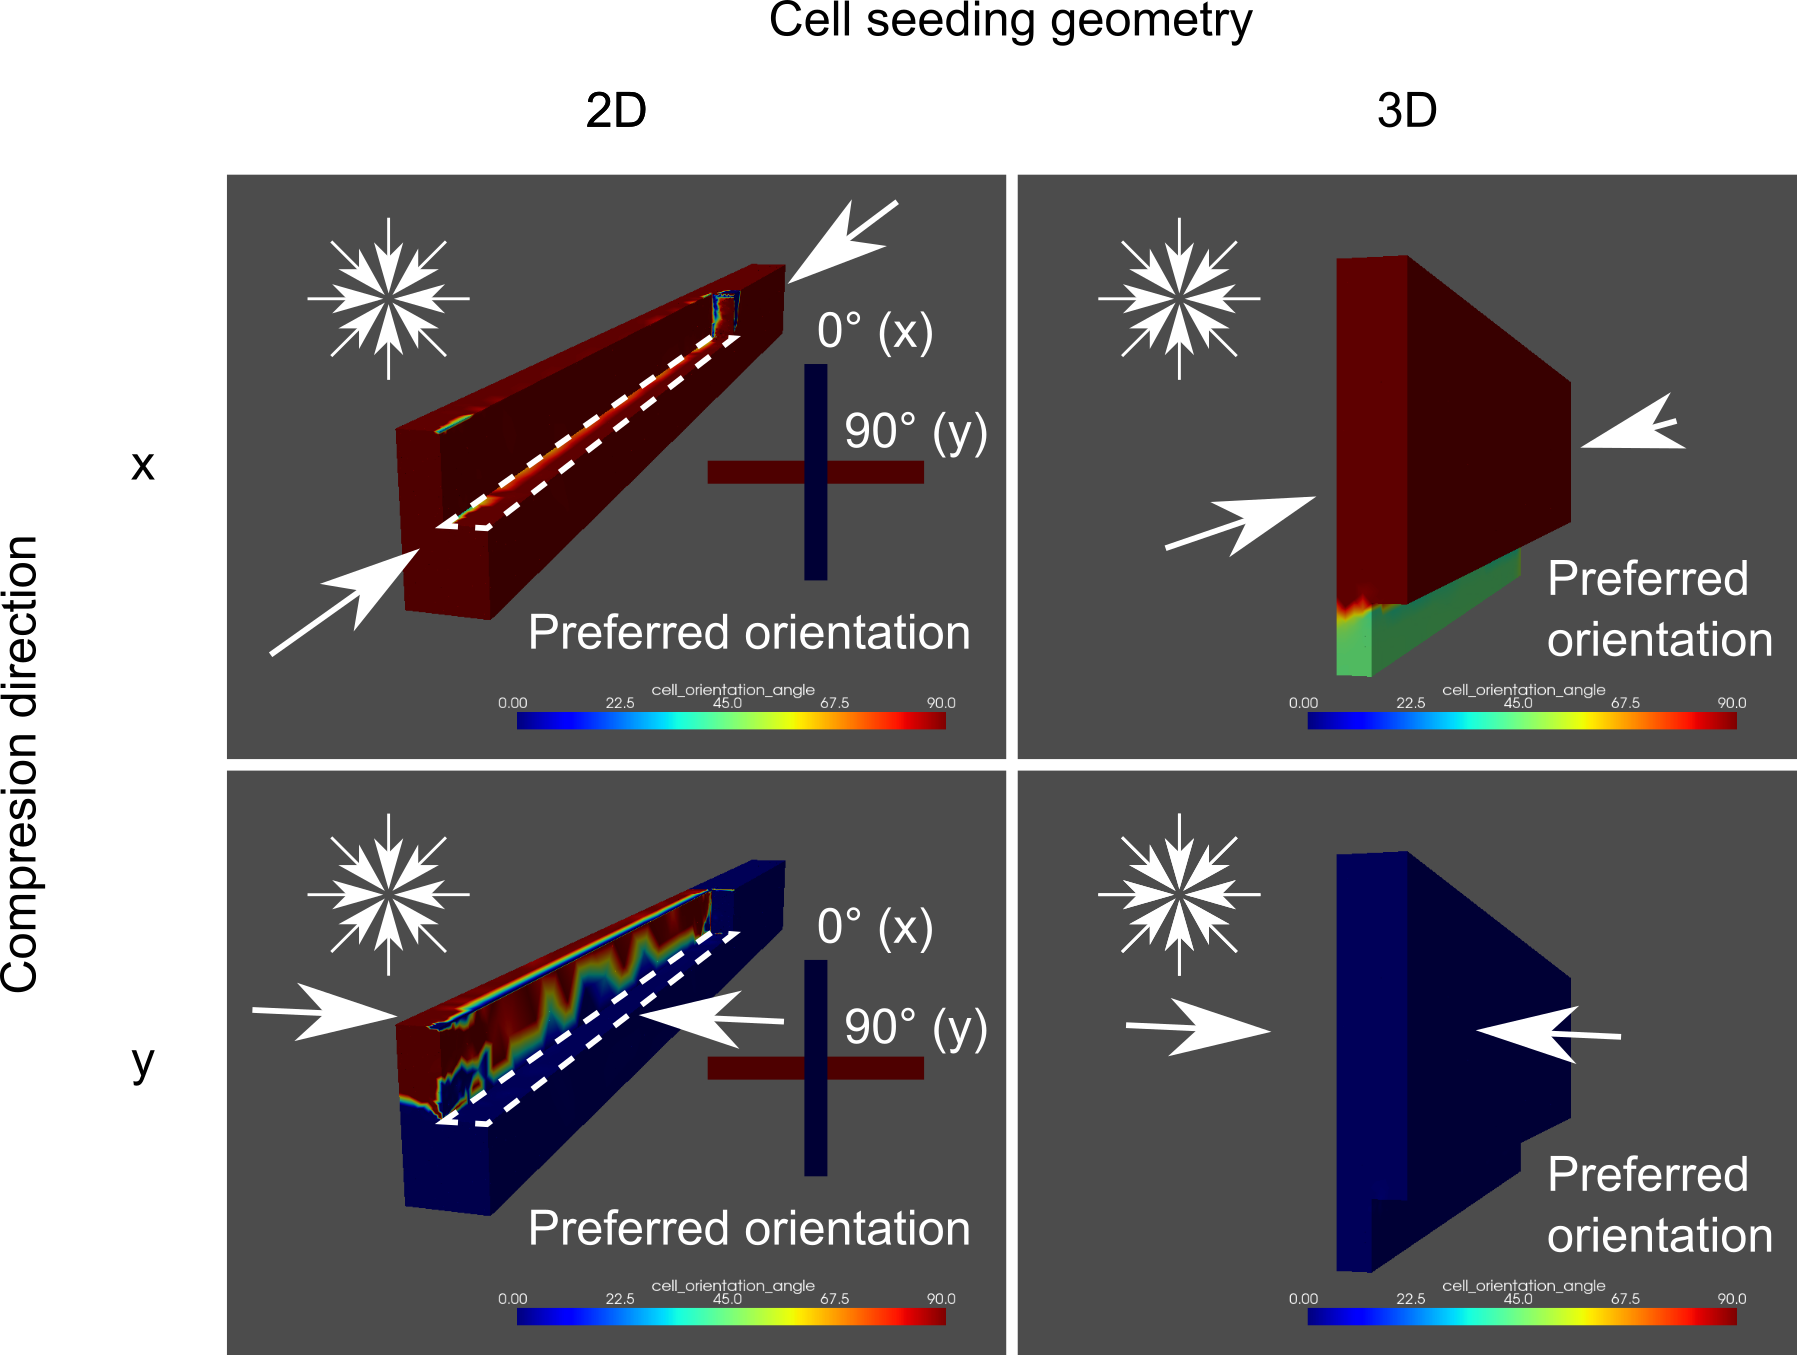
\includegraphics[width=1.0\textwidth]{figures/figure_11_cell_orientation_combined.png}
\caption[Cell orientation with combined cues]{Analysis of modelled cell orientation when combination the cues arising from self-contraction and mechanical stimulation. This figure reports the orientation associated with least overall compression (according to eq. \ref{eq_maximization_procedure}) arising by combination of cellular self-contraction and external mechanical stimulation, in both 2D and hydrogel 3D seeding geometries, for mechanical stimulation along the grooves ($x$) or perpendicular ($y$). The dashed area in the 2D geometry designates the bottoms of the grooves primarily imaged.}
\label{fig_cell_orientation_combined}
}
\end{figure}


Next, we add the strain cues arising from cellular contraction and ensuing self-condensation on the one hand and cyclic mechanical stretch on the other. To combine the cueing effects of such physically distinct processes, we use the strain avoidance maximization procedure outlined by eq. \ref{eq_maximization_procedure}, which in turn is based on the elementary strain elongation addition law given by eq. \ref{eq_strain_addition}, which is a rough, empirical recapitulation of lumped cellular behavior. Given its central importance, eq. \ref{eq_strain_addition} is also given as eq. 1 in the main text.

Fig. \ref{fig_cell_orientation_combined} shows the orientation modelled to minimze total perceived compression strain by the cells in four prototypical scenarii: Compression along the grooves, or perpendicular to them, applied to either cells seeded 3D in a hydrogel or 2D on top of the flat surfaces of the PDMS. For the 2D configuration, the mechanical stimulation prevails mostly and cellular orientation is approximately perpendicular to the direction of applied cyclic stimulation, at least in the primary zone of interest on the bottom of the grooves. In 3D, the strain avoidance addition provides an interesting contrasted result.  Firstly, for stimulation perpendicular to the grooves, the alignment cues match up to strong alignment along the grooves. Secondly, and most importantly, for stimulation along the grooves, the alignment cues are conflicting. Indeed, mechanical stimulation alone would cause alignment perpendicular to the grooves, whereas self-condensation would provide alignment along the grooves. Within the groove volume, an intermediate orientation results, with an alignment angle in the vicinity of 45°. This observation of intermediate orientation with conflicting cues is at the heart of engineering oblique cellular orientation as proposed here.

Finally, we consider the stretch ratio (eq. \ref{eq_r}) to define the local strain anisotropy as a measure of the strength of the overall orientation cue. The stretch in this case arises from the maximum and minimum elongation as defined by strain addition (eq. \ref{eq_strain_addition}) in different directions in the $xy$-plane.  

\begin{figure}
\center{
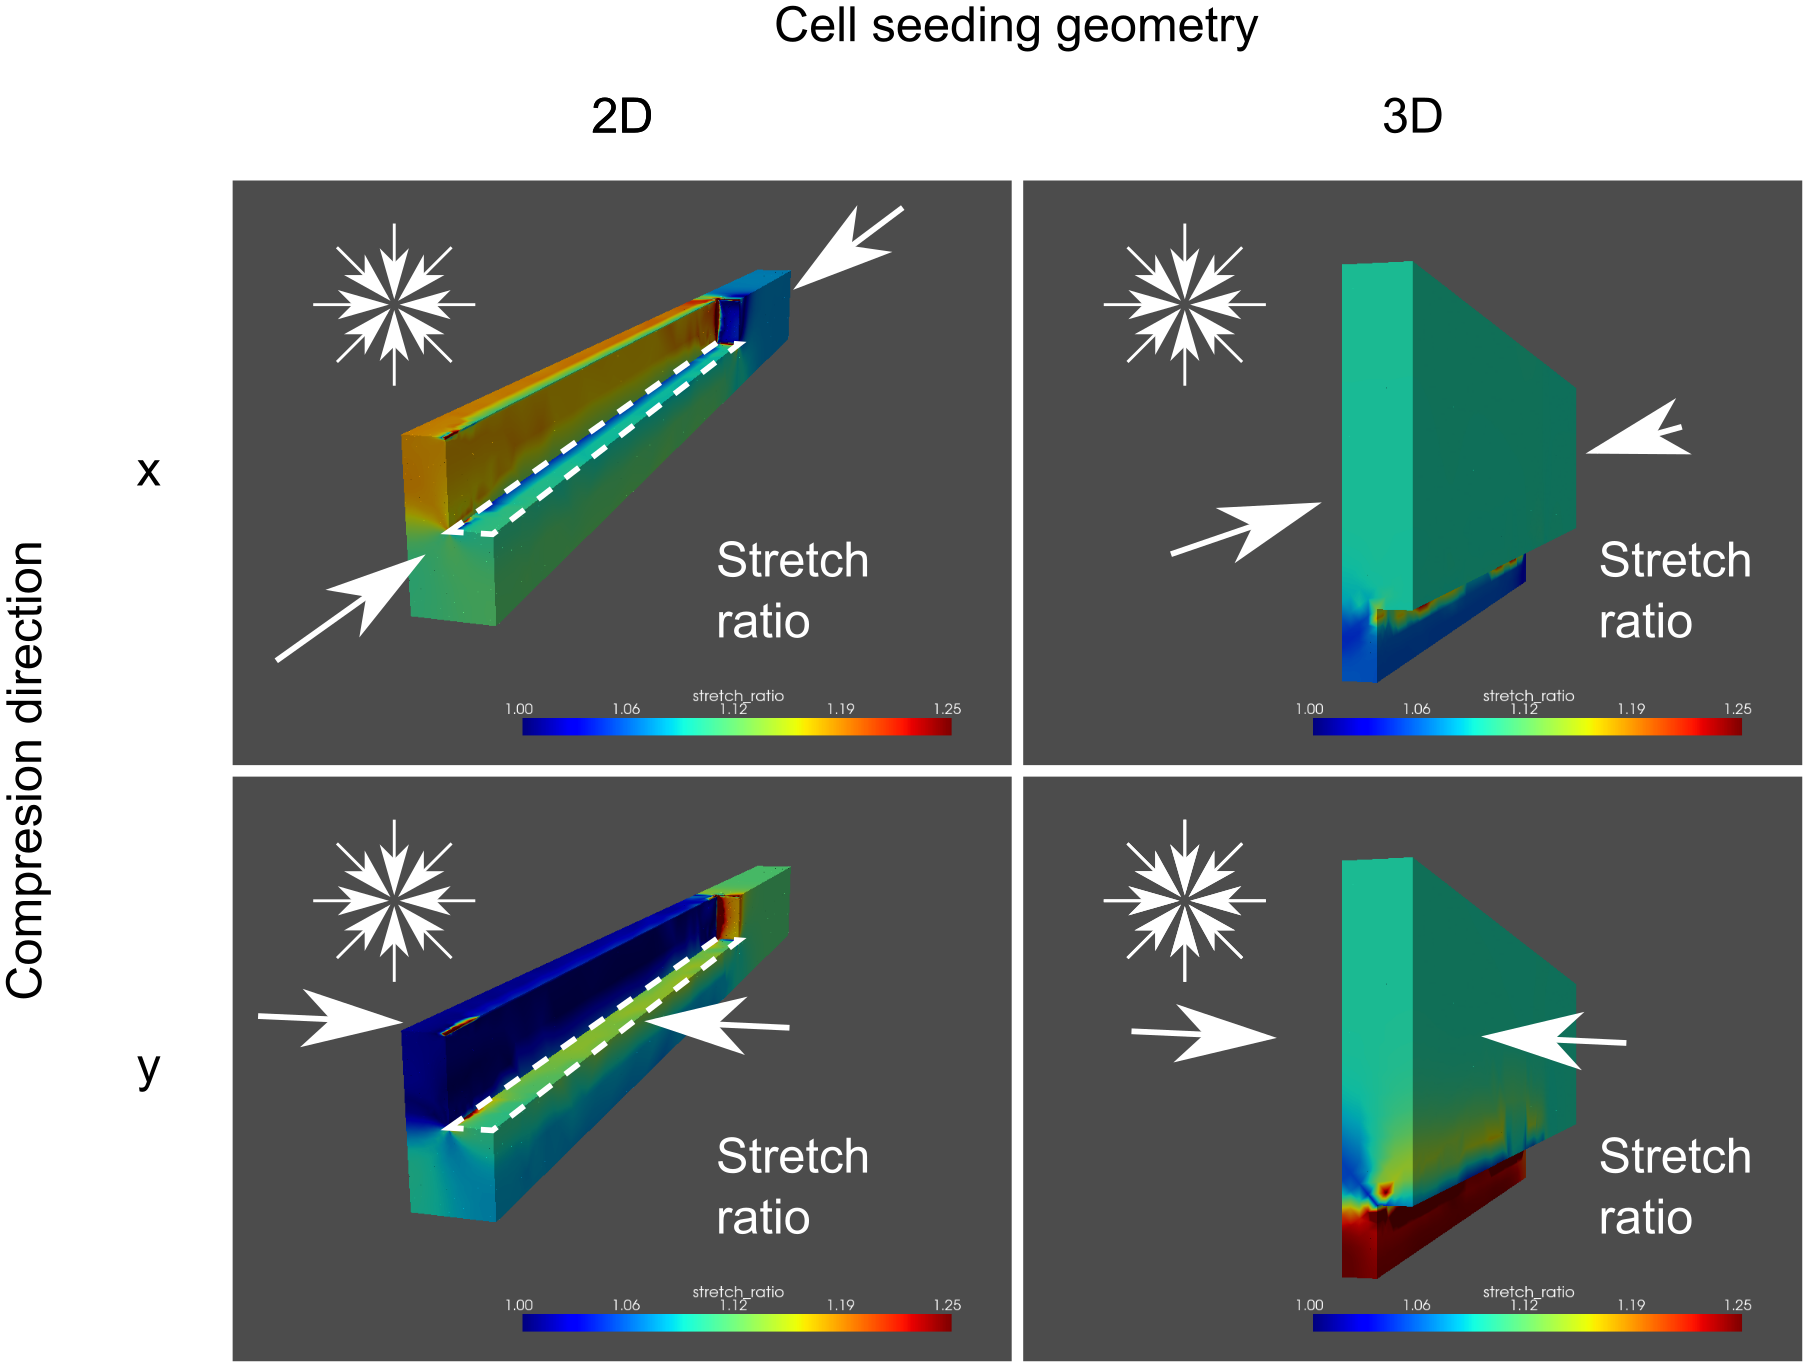
\includegraphics[width=1.0\textwidth]{figures/figure_12_stretch_ratio_combined.png}
\caption[Stretch with combined cues]{}
\label{fig_stretch_ratio_combined}
}
\end{figure}


\section{Discussion}

In this supplementary, we describe a simple simulation based on linear elasticity and strain avoidance to model cell orientation behaviour. In particular, we provide a lumped strain avoidance model permitting to qualitatively understand cell orientation in the framework of conflicting cues.

The model is voluntarily simplistic, and it is worth stressing a few major limitations. The first limitation concern the elasticity simulation itself. The assumption of linear, isotropic elasticity is well warranted for the PDMS structures, because PDMS exhibits extended linear elasticity, and also because the deformations are relatively small. For the hydrogel, it is at best a qualitative assumption. Hydrogels typically exhibit non-linear elastic responses, and upon self condensation due to cellular action, we also expect isotropicity to be lost. In this sense, the model given here cannot be quantitative in an absolute sense, it rather portrays orders of magnitude of strains involved and fundamental processes. Similarly, the lumped stress avoidance addition model (eq. \ref{eq_strain_addition} and the associated maximization procedure given by eq. \ref{eq_maximization_procedure}) is based on a phenomenological, ultimately empirical approach. It has a  mechanistic basis in more complex models of stress fiber dynamics, which indeed predict redistribution of actin monomers away from regions being compressed due to thermodynamic mechanisms operating towards keeping the strain per actomyosin unit constant\cite{chen_role_2018}. These cellular processes are however exceedingly complex and involve not only elastic components, but also molecular modification and regional diffusion\cite{vigliotti_thermodynamically_2016}. The lumped model used here is obviously far from capturing the details of these dynamics. It is for instance not meant to account for  subtle, and poorly understood frequency dependence of the strain avoidance response\cite{chen_role_2018}. As much as simplicity comes at the cost of neglecting mechanistic details, as much it has the advantage to be directly usable for engineering purposes: state-of-the-art software today allows for straightforward evaluation of linear elasticity problems such as the ones posed here, and strain addition modelling can easily be implemented once the strain matrices are known, using very limited amounts of custom code.

Further, the very notion of strain avoidance most likely does not capture all aspects of cell alignment. For instance, as evident from Fig. \ref{fig_cell_orientation_self_condensation}, in the 2D geometry, strain avoidance by itself should have relatively little influence on cell orientation - substantial strain asymmetry is present only in very restricted areas near the edges. In contradiction, even in the complete absence of mechanical stimulation, we observe important cell alignment under these conditions (not shown). We thus conclude that to be more complete, one certainly would have to take into account other cell alignment mechanisms such as topographical guidance including at subcellular scales\cite{leclech_cellular_2020}, chemical gradients\cite{wu_modeling_2011}, matrix rearrangement and alignment to anisotropically aranged matrix\cite{bourget_alignment_2013}, and possibly long-range mechanical communication between cells\cite{humphries_mechanical_2017}.

Despite the numerous simplifications, in terms of phenomenological observation, the model captures and tentatively explains key empirical observations. First, when directly seeded onto the relatively stiff PDMS substrates ("2D geometry"), the mechanical stimulation has an overwhelming influence compared to geometrical alignment. Our model suggests that this is because the cells are only able to impart small strains on the PDMS, since they are themselves much softer than their substrate. It appears therefore natural that the substantially larger external stretch signal almost completely dominates local cell orientation in the 2D configuration. In the 3D hydrogel environment, the situation is different, the cells are anticipated to be able to cause large-scale deformation, especially in the longer term where pore fluid displacement makes local compaction of the polymer strands possible with effective Poisson coefficients substantially below 0.5\cite{braschler_soft_2015}. This leads to the well-known phenomena of hydrogel self-condensation\cite{sawhney_slow_2002} observed for instance in engineered heart tissue EHT constructs\cite{zimmermann_tissue_2002}, but also causes the deformations imparted by the cells to be fully competitive with externally imposed mechanical stretch. The strain addition model given here then predicts intermediate orientations, in agreement with empirical observations and in line with our primary target of engineer oblique cell orientation.

There is a fundamental importance in the assumed non-linearity of the cellular response. Indeed, if the cellular response were strictly linear, cyclic mechanical stimulation with symmetrical compression and extension phases would have no net effect on the cells, in obvious conflict with our, but also essentially all other previously reported empirical results\cite{chen_role_2018}. The importance of non-linearity goes however beyond this. If strain addition were purely linear, symmetrical strain matrices would have to be added directly, yielding again symmetrical strain matrices. However, symmetrical matrices have particular properties, among which are eigenvectors for distinct eigenvalues at right angles\cite{beresford_symmetric_1980}. Therefore, in 2D observations, one would expect there to be either a single preferred direction or total isotropy and thus randomness in orientation. On the contrary, non-linear strain addition in the presence of two orthogonal cues predicts there to be generally two favorite directions when adding two strains, towards the stronger cue, but with an angle between them that can range from 0° to 90°. In the confocal images used for alignment quantification, at second sight, this is generally the case. In conditions where some degree of oblique alignment is found, in fact two favorite directions of stress fibers are observed, and they are symmetrical with regard to the externally imposed stronger cue. In our case, this is at roughly $\pm45$° for the 3D oblique alignment, and at around $\pm5°$ off the mechanically imposed orientation in case of the conflicting 2D seeding geometry. 

It is maybe worth adventuring to sketch a thermodynamic basis for the inferred non-linearity and specific relevance of the compressive part of the mechanical stimulation cycle. If indeed cell reorientation reflects elementary kinetics of cytoskeleton polymerization-depolymerization\cite{vigliotti_thermodynamically_2016}, with the free energy of the polymerized state being dependent on strain, but the transition state relatively independent on the mechanical state\cite{vigliotti_thermodynamically_2016}, then the depolymerization rate will depend much more heavily on the mchanical state than the polymerization rate. Schematically, one looks then at the net effect of a roughly constant polymerization rate \textit{vs.} depolymerization depending exponentially on applied compression\cite{vigliotti_thermodynamically_2016}. Overall, this is a potentially highly non-linear process, with a fundamental asymmetry regarding compression and extension. Indeed, even in extreme extension, in this thermodynamic view net stress fiber growth is limited by the constant intrinsic polymerization rate. On the contrary, depolymerization under compression can become very large, leading to potential net depolymerization many times the maximum polymerization rate. In other words, in this case the extension phase cannot compensate for the powerful action of the compression phase. These schematic thermodynamic lines of reasoning are thus in line with our model suggestions that place particular importance on compression and non-linearity. 

The modelling here also raises a series of interesting questions beyond the results obtained. In more extended experimental series, one could aim at defining better the strain addition law. The model of strain addition given here suggests that depending on the relative magnitude of external cyclic stretch, alignment angles between fully geometrical alignment and full stretch-dominated alignment can be obtained. The exact dependency of the alignment angle on the stretch magnitude could be used to define more precisely the strain addition law; eq. \ref{eq_strain_addition} is an educated guess compatible with the results observed here, but one could possibly refine its form and certainly the addition coefficient $n$. Also, as outlined above, we obtain two, rather than one defined favorite orientation angle due to the non-linearity of the model. A unique oblique alignment axis may be more preferrable in certain applications, one would probably need to add a third cue making one of the two orientations less favorable. In other applications, spatially inhomogeneous alignment may be desired, here, one could exploit local shaping of the strain field by local stimulation or alternatively use specific engineering of stress concentration to obtain spatially inhomogeneous compression directions and thus cell orientation.


\bibliographystyle{classes/siam_with_author_repetition}
\bibliography{supplementary_library.bib}
 
 

\end{document} 